\documentclass[11pt,letterpaper]{article}

% ============================================================================
% PACKAGES
% ============================================================================
\usepackage[utf8]{inputenc}
\usepackage[T1]{fontenc}
\usepackage{helvet}
\renewcommand{\familydefault}{\sfdefault}
\usepackage[margin=0.85in, headheight=28pt]{geometry}
\usepackage{graphicx}
\usepackage{xcolor}
\usepackage{tikz}
\usepackage{tcolorbox}
\usepackage{booktabs}
\usepackage{enumitem}
\usepackage{hyperref}
\usepackage{fancyhdr}
\usepackage{titlesec}
\usepackage{multicol}
\usepackage{listings}
\usepackage{upquote}
\usepackage{amsmath,amssymb}
\usepackage{pgfplots}
\usepackage{array}
\usepackage{longtable}

% Ragged-right paragraph columns to prevent word spacing issues
\newcolumntype{L}[1]{>{\raggedright\arraybackslash}p{#1}}

% Increase vertical spacing between table rows for readability
\renewcommand{\arraystretch}{1.4}
\usepackage{colortbl}
\usepackage{pifont}
\usepackage{setspace}
\usepackage{parskip}
\usepackage{caption}
\usepackage{tabularx}

\pgfplotsset{compat=1.18}
\usetikzlibrary{shapes.geometric, arrows.meta, positioning, calc, decorations.pathreplacing, backgrounds, fit, shadows.blur, matrix, patterns, fadings, shadings}

% ============================================================================
% COLOR DEFINITIONS - Fractured Authority Theme (Institutional Erosion)
% ============================================================================
% Primary: Deep slate - institutional weight, government authority
\definecolor{slateprimary}{HTML}{1E293B}
\definecolor{slatedark}{HTML}{0F172A}
\definecolor{slatemid}{HTML}{334155}
% Secondary: Weathered bronze/stone - aged institutions, legacy systems
\definecolor{bronzeweathered}{HTML}{92735F}
\definecolor{stonegray}{HTML}{78716C}
\definecolor{patinabronze}{HTML}{A68B6A}
% Accent: Fracture amber/orange - stress points, erosion, warning
\definecolor{fractureamber}{HTML}{B86B3A}
\definecolor{stressorange}{HTML}{B07A35}
\definecolor{erosionyellow}{HTML}{C8923A}
% Alert: Deep burgundy/wine - critical vulnerabilities
\definecolor{burgundydeep}{HTML}{881337}
\definecolor{wineaccent}{HTML}{8A2D42}
% Verification: Teal - adaptation, verification, hope
\definecolor{verifyteal}{HTML}{0F766E}
\definecolor{adaptteal}{HTML}{4A9A8B}
% Neutrals
\definecolor{coolgray}{HTML}{64748B}
\definecolor{lightgray}{HTML}{F1F5F9}
\definecolor{textlight}{HTML}{CBD5E1}
\definecolor{gridlight}{HTML}{E2E8F0}
% Standard ETRA header band gold (consistent across all projection reports)
% Note: barriergold now matches instgold (#B7950B) for consistent ETRA header bands
\definecolor{barriergold}{HTML}{B7950B}

% ============================================================================
% HYPERREF SETUP
% ============================================================================
\hypersetup{
  colorlinks=true,
  linkcolor=slatemid,
  urlcolor=verifyteal,
  pdftitle={AI Agents and Institutional Erosion of Intelligence Monopolies},
  pdfauthor={Emerging Technology Risk Assessment}
}

% ============================================================================
% SPACING AND TYPOGRAPHY
% ============================================================================
\setstretch{1.15}
\setlength{\parskip}{0.5em}
\setlist{nosep, leftmargin=1.5em, itemsep=0.3em}
\raggedbottom

% ============================================================================
% PAGE STYLE - Fracture pattern accent (institutional erosion theme)
% ============================================================================
\pagestyle{fancy}
\fancyhf{}
\fancyhead[L]{%
  \begin{tikzpicture}[baseline=-0.5ex]
    % Fractured seal fragment pattern
    \fill[bronzeweathered, opacity=0.6] (0,0.12) -- (0.15,0.18) -- (0.12,0.06) -- cycle;
    \fill[bronzeweathered, opacity=0.5] (0.18,0.1) -- (0.32,0.16) -- (0.28,0.04) -- cycle;
    \draw[fractureamber, opacity=0.7, line width=0.6pt] (0.12,0.12) -- (0.22,0.08);
    \draw[fractureamber, opacity=0.5, line width=0.4pt] (0.08,0.06) -- (0.18,0.14);
    \fill[fractureamber, opacity=0.9] (0.36,0.12) circle (0.04);
  \end{tikzpicture}
  \hspace{0.5em}\textcolor{slateprimary}{\textsf{\small ETRA-2026-IC-001}}%
}
\fancyhead[R]{\textcolor{coolgray}{\textsf{\thepage}}}
\fancyfoot[C]{\textcolor{coolgray}{\footnotesize\textsf{Emerging Technology Risk Assessment \textbar{} Institutional Erosion}}}
\renewcommand{\headrulewidth}{0pt}
\renewcommand{\footrulewidth}{0pt}

\fancyheadoffset{0pt}
\setlength{\headheight}{32pt}

% ============================================================================
% SECTION FORMATTING - Fractured authority style with erosion accent
% ============================================================================
\titleformat{\section}
  {\normalfont\LARGE\bfseries\color{slatedark}}
  {\thesection}{0.8em}{}[\vspace{-0.3em}{\color{bronzeweathered}\rule{\textwidth}{1.5pt}\hspace{-\textwidth}\color{fractureamber}\rule{3cm}{1.5pt}}]
\titleformat{\subsection}
  {\normalfont\Large\bfseries\color{slateprimary}}
  {\thesubsection}{0.6em}{}
\titleformat{\subsubsection}
  {\normalfont\large\color{stonegray}\bfseries}
  {\thesubsubsection}{0.5em}{}

\titlespacing*{\section}{0pt}{3ex plus 1ex minus .2ex}{2ex plus .2ex}
\titlespacing*{\subsection}{0pt}{2.5ex plus 1ex minus .2ex}{1.5ex plus .2ex}

\setcounter{tocdepth}{2}

% ============================================================================
% TCOLORBOX ENVIRONMENTS - Fractured Authority Theme
% ============================================================================
\tcbuselibrary{skins,breakable,hooks}

\newtcolorbox{keybox}[1][Key Finding]{
  enhanced, breakable,
  colback=slatemid!8, colframe=slatemid,
  colbacktitle=slatemid, coltitle=white,
  fonttitle=\bfseries\sffamily,
  title={\ding{72}\hspace{0.5em}#1},
  boxrule=0pt, leftrule=4pt, arc=0pt, outer arc=0pt,
  left=12pt, right=12pt, top=8pt, bottom=8pt
}

\newtcolorbox{warnbox}[1][Warning]{
  enhanced, breakable,
  colback=stressorange!10, colframe=stressorange,
  colbacktitle=stressorange, coltitle=white,
  fonttitle=\bfseries\sffamily,
  title={\ding{74}\hspace{0.5em}#1},
  boxrule=0pt, leftrule=4pt, arc=0pt, outer arc=0pt,
  left=12pt, right=12pt, top=8pt, bottom=8pt
}

\newtcolorbox{criticalbox}[1][Critical]{
  enhanced, breakable,
  colback=burgundydeep!10, colframe=burgundydeep,
  colbacktitle=burgundydeep, coltitle=white,
  fonttitle=\bfseries\sffamily,
  title={\ding{74}\hspace{0.5em}#1},
  boxrule=0pt, leftrule=4pt, arc=0pt, outer arc=0pt,
  left=12pt, right=12pt, top=8pt, bottom=8pt
}

\newtcolorbox{recbox}[1][Recommendation]{
  enhanced, breakable,
  colback=verifyteal!10, colframe=verifyteal,
  colbacktitle=verifyteal, coltitle=white,
  fonttitle=\bfseries\sffamily,
  title={\ding{51}\hspace{0.5em}#1},
  boxrule=0pt, leftrule=4pt, arc=0pt, outer arc=0pt,
  left=12pt, right=12pt, top=8pt, bottom=8pt
}

\newtcolorbox{infobox}[1][Note]{
  enhanced, breakable,
  colback=adaptteal!10, colframe=adaptteal!80!slatedark,
  colbacktitle=adaptteal!80!slatedark, coltitle=white,
  fonttitle=\bfseries\sffamily,
  title={\ding{73}\hspace{0.5em}#1},
  boxrule=0pt, leftrule=4pt, arc=0pt, outer arc=0pt,
  left=12pt, right=12pt, top=8pt, bottom=8pt
}

\newtcolorbox{defbox}[1][Definition]{
  enhanced, breakable,
  colback=bronzeweathered!12, colframe=bronzeweathered,
  colbacktitle=bronzeweathered, coltitle=white,
  fonttitle=\bfseries\sffamily,
  title={\ding{70}\hspace{0.5em}#1},
  boxrule=0pt, leftrule=4pt, arc=0pt, outer arc=0pt,
  left=12pt, right=12pt, top=8pt, bottom=8pt
}

\newtcolorbox{scenariobox}[1][Scenario]{
  enhanced, breakable,
  colback=stonegray!8, colframe=stonegray,
  colbacktitle=stonegray, coltitle=white,
  fonttitle=\bfseries\sffamily,
  title={\ding{118}\hspace{0.5em}#1},
  boxrule=0pt, leftrule=4pt, arc=0pt, outer arc=0pt,
  left=12pt, right=12pt, top=8pt, bottom=8pt
}

% ============================================================================
% DOCUMENT
% ============================================================================
\begin{document}

% ============================================================================
% TITLE PAGE - Fractured Institutional Seal Visualization
% ============================================================================
\begin{titlepage}

\begin{tikzpicture}[remember picture, overlay]
  % Background - deep slate
  \fill[slatedark] (current page.north west) rectangle (current page.south east);

  % Weathered texture background pattern (institutional decay aesthetic)
  \begin{scope}[shift={(current page.center)}, opacity=0.04]
    % Horizontal striations suggesting aging/weathering
    \foreach \y in {-12,-10,...,12} {
      \draw[bronzeweathered, line width=0.3pt] (-10,\y) -- (10,\y);
    }
    % Vertical cracks pattern
    \foreach \x in {-8,-4,0,4,8} {
      \draw[fractureamber, line width=0.4pt] (\x,-12) -- ({\x+0.5},12);
    }
  \end{scope}

  % Main visualization - IC Shield Under Siege (Simplified)
  \begin{scope}[shift={([xshift=-0.5cm, yshift=3.5cm]current page.center)}]

    % Subtle radial gradient - depth cue
    \shade[inner color=white, outer color=slatedark, opacity=0.08] (0,0) circle (5.5cm);

    % OUTER RING - Collection layer (IC Agency perimeter)
    \draw[bronzeweathered, opacity=0.3, line width=16pt] (0,0) circle (4.5cm);
    \draw[bronzeweathered, opacity=0.6, line width=2pt] (0,0) circle (4.5cm);
    % Ring label
    \node[textlight, opacity=0.35, font=\fontsize{7}{7}\selectfont\sffamily] at (270:5.4cm) {COLLECTION};

    % IC Agency nodes positioned ON the outer ring
    \foreach \angle/\label in {90/NSA, 140/FBI, 180/DIA, 220/NGA, 270/NRO, 320/DHS, 0/ODNI, 50/CIA} {
      \fill[slatemid] (\angle:4.5cm) circle (0.55cm);
      \draw[bronzeweathered, opacity=0.8, line width=1.5pt] (\angle:4.5cm) circle (0.55cm);
      \node[white, font=\fontsize{8}{8}\selectfont\bfseries] at (\angle:4.5cm) {\label};
    }

    % MIDDLE RING - Analysis layer
    \draw[stonegray, opacity=0.25, line width=12pt] (0,0) circle (3cm);
    \draw[stonegray, opacity=0.5, line width=1.5pt] (0,0) circle (3cm);
    % Ring label
    \node[textlight, opacity=0.35, font=\fontsize{7}{7}\selectfont\sffamily] at (270:3.5cm) {ANALYSIS};

    % INNER RING - Verification layer (the protective barrier)
    \draw[verifyteal, opacity=0.25, line width=8pt] (0,0) circle (1.9cm);
    \draw[verifyteal, opacity=0.5, line width=1.5pt] (0,0) circle (1.9cm);
    % Ring label
    \node[textlight, opacity=0.35, font=\fontsize{7}{7}\selectfont\sffamily] at (270:2.3cm) {VERIFICATION};

    % === CENTRAL CORE - Decision (protected by verification) ===
    \shade[inner color=patinabronze!60, outer color=patinabronze!10, opacity=0.3] (0,0) circle (1.5cm);
    \fill[slatedark] (0,0) circle (1.2cm);
    \fill[patinabronze, opacity=0.9] (0,0) circle (0.9cm);
    \draw[bronzeweathered, line width=3pt] (0,0) circle (0.9cm);
    \node[white, font=\fontsize{9}{9}\selectfont\bfseries] at (0,0) {DECISION};

    % Teal verification aura protecting the decision core
    \draw[verifyteal, opacity=0.6, line width=3pt] (0,0) circle (1.08cm);
    \draw[verifyteal, opacity=0.3, line width=5pt] (0,0) circle (1.35cm);

  \end{scope}

  % Document classification bar (standard ETRA gold - consistent across all reports)
  \fill[barriergold] ([yshift=-1.5cm]current page.north west) rectangle ([yshift=-2.2cm]current page.north east);
  \node[slatedark, font=\small\bfseries\sffamily] at ([yshift=-1.85cm]current page.north) {PROJECTION REPORT \textbar{} ETRA-2026-IC-001 \textbar{} FEBRUARY 2026};

  % Title block (bottom left)
  \node[anchor=south west, text width=14cm] at ([xshift=1.5cm, yshift=3cm]current page.south west) {
    {\fontsize{11}{13}\selectfont\color{fractureamber}\sffamily EMERGING TECHNOLOGY RISK ASSESSMENT}\\[0.8cm]
    {\fontsize{32}{38}\selectfont\bfseries\color{white}AI Agents and}\\[0.2cm]
    {\fontsize{32}{38}\selectfont\bfseries\color{white}Institutional Erosion of}\\[0.2cm]
    {\fontsize{32}{38}\selectfont\bfseries\color{white}Intelligence Monopolies}\\[0.6cm]
    {\large\color{textlight}\sffamily The Verification Pivot: How Autonomous AI Transforms the IC}
  };

  % Metadata block (bottom right)
  \node[anchor=south east, text width=6cm, align=right] at ([xshift=-1.5cm, yshift=3cm]current page.south east) {
    \color{textlight}\small\sffamily
    \textbf{Document Type:} Policy Research\\[0.2em]
    \textbf{Time Horizon:} 2026--2030\\[0.2em]
    \textbf{License:} MIT / Unlicense\\[0.2em]
    \textbf{Version:} 2.0
  };

  % Vertical accent line (weathered bronze)
  \draw[bronzeweathered, line width=2pt] ([xshift=1.5cm, yshift=3cm]current page.south west) -- ([xshift=1.5cm, yshift=10.5cm]current page.south west);

\end{tikzpicture}
\end{titlepage}

% ============================================================================
% EXECUTIVE SUMMARY
% ============================================================================
\thispagestyle{empty}
\vspace*{0.5cm}

% Mini header visualization - fractured seal fragments
\noindent\begin{tikzpicture}
  \fill[slatedark] (0,0) rectangle (\textwidth, 0.15);
  % Fracture pattern across header
  \foreach \x in {0.5,1.2,...,16.5} {
    \fill[bronzeweathered, opacity=0.4] (\x, 0.075) circle (0.04);
  }
  % Stress points
  \fill[fractureamber, opacity=0.8] (4, 0.075) circle (0.05);
  \fill[fractureamber, opacity=0.8] (12, 0.075) circle (0.05);
\end{tikzpicture}

\vspace{0.3cm}
\begin{center}
{\color{slatedark}\Large\bfseries Executive Summary}
\end{center}
\vspace{0.15cm}

\begin{tcolorbox}[enhanced, colback=lightgray, colframe=slatemid!50, boxrule=1pt, arc=3pt,
  left=10pt, right=10pt, top=10pt, bottom=10pt]
This projection examines how autonomous AI agents are eroding the traditional advantages of national intelligence communities, particularly the U.S. Intelligence Community (IC). We analyze current technological capabilities through February 2026, project likely institutional impacts through 2030, and examine how intelligence organizations must adapt to maintain epistemic authority in an AI-saturated information environment.
\end{tcolorbox}

\vspace{0.2cm}

\begin{keybox}[Central Thesis: The Verification Pivot]
The IC is transitioning from an era of \textbf{Information Scarcity}---where advantage derived from superior collection capabilities---to an era of \textbf{Epistemic Contamination}---where advantage derives from superior verification capabilities. This represents the most significant shift in intelligence dynamics since the advent of signals intelligence.

\vspace{0.5em}
\textbf{Secondary Thesis: From Secrecy to Provenance}

In an AI-saturated environment, \textit{classification alone} is no longer a reliable proxy for decision value. Intelligence products derive value from (1) protecting sources and methods \textit{and} (2) providing high-integrity, auditable provenance for key claims.
\end{keybox}

\begin{infobox}[Note on IC Internal Provenance]
Classified systems already maintain chain-of-custody, compartmentation, and audit trails. The thesis is not that the IC lacks provenance mechanisms, but that \textbf{verification and integrity mechanisms must become first-class properties} of intelligence products consumed by decision-makers---not merely security features for access control. The shift is from ``who can see this'' to ``why should this be believed.''
\end{infobox}

\vspace{0.1cm}

\begin{keybox}[Key Findings]
\begin{enumerate}
  \item \textbf{[E] The Democratization of Tradecraft}: AI agents have effectively ``automated the Handler.'' Tradecraft that once required sovereign state infrastructure is now a commodity.
  \item \textbf{[E]} The IC faces a dual crisis: \textbf{Process DoS} (investigative capacity overwhelmed) and an \textbf{Attribution-Intent Gap} (inability to establish human intent behind agent actions)
  \item \textbf{[E]} Current collection-centric metrics become counterproductive in an environment of epistemic contamination
  \item \textbf{[S]} Success in 2026-2030 will be measured by the ability to maintain an ``Epistemic Clean Room''---a verified environment for decision-making
  \item \textbf{[E]} The ``Plausible Deniability 2.0'' dynamic will strain existing legal frameworks for state responsibility
  \item \textbf{[S]} Without adaptation, the IC risks becoming a high-cost verification bottleneck rather than a strategic advantage
\end{enumerate}
\end{keybox}

\vspace{0.2cm}

\begin{warnbox}[Scope Limitations]
This document analyzes capabilities and institutional dynamics for defensive policy purposes. It does not provide operational guidance and explicitly omits technical implementation details that could enable harm. Analysis focuses on how autonomous agents change intelligence dynamics, not on intelligence methods generally.
\end{warnbox}

\vspace{0.2cm}

\begin{infobox}[Independent Work]
This report is independent research. It is not affiliated with, produced by, or endorsed by any government agency, think tank, or official institution. The ``ETRA'' identifier is a document formatting convention, not an organizational identity. Analysis draws on publicly available academic and policy literature.
\end{infobox}

\vspace{0.2cm}

% ============================================================================
% EXECUTIVE TAKEAWAYS
% ============================================================================
\begin{center}
{\color{slatedark}\Large\bfseries Executive Takeaways}
\end{center}

\begin{defbox}[5 Non-Negotiable Assumptions]
\begin{enumerate}
  \item \textbf{The capability floor has risen permanently} --- Low-cost access to frontier models can automate major components of tradecraft---research, targeting, persona drafting, multilingual engagement---reducing manpower barriers even when operational constraints remain.
  \item \textbf{Collection without verification is now a liability} --- In targeted collection environments, agent-generated decoys could plausibly outnumber authentic human signals by $\sim$3--30$\times$. Traditional signal-to-noise filters become unreliable.
  \item \textbf{Attribution of intent is structurally harder} --- The ``Delegation Defense'' (blaming autonomous agent behavior) provides plausible deniability for state actors using AI agents.
  \item \textbf{Institutional speed cannot match adversary iteration} --- Adversaries iterate at software speed; IC adoption is constrained by procurement, authorities, and assurance requirements.
  \item \textbf{[O] Verification workforce is contracting} --- Confirmed IC staffing reductions: NSA met 2,000-person reduction (Dec 2025); ODNI cut to $\sim$1,300 under ``ODNI 2.0,'' dissolving the Foreign Malign Influence Center; CIA shrinking $\sim$1,200 positions; $\sim$8\% annual DOD budget cuts affect all military intelligence.
\end{enumerate}
\end{defbox}

\vspace{0.1cm}

\begin{keybox}[5 Most Likely Impact Paths]
\begin{center}
\small
\begin{tabular}{L{3cm}L{5cm}L{4.5cm}}
\toprule
\textbf{Path} & \textbf{Mechanism} & \textbf{Primary Victims} \\
\midrule
Process DoS & Agent-generated leads, hyper-specific FOIA requests, synthetic tips overwhelm capacity & FBI, DHS, investigative agencies \\
Epistemic Contamination & Synthetic content pollutes OSINT/GEOINT, eroding ``ground truth'' & All-source analysts, ODNI \\
Attribution-Intent Gap & States claim agents ``autonomously derived'' criminal methods & Legal/policy leadership, State Dept \\
Algorithmic Capture & Compromise of AI systems used by leadership biases intelligence products & ODNI, CIA, NSC \\
Nano-Smurfing Evasion & Sub-threshold procurement of dual-use items evades monitoring & Treasury, DOE, proliferation watchers \\
\bottomrule
\end{tabular}
\end{center}
\end{keybox}

\vspace{0.1cm}

\begin{infobox}[Success Criteria]
\begin{center}
\small
\begin{tabular}{L{4cm}L{4.2cm}L{4.2cm}}
\textbf{90 days} & \textbf{180 days} & \textbf{1 year} \\
\midrule
Verification metric defined; red-teams run; no unvetted AI in leadership workflows & Provenance prototype; detection sharing operational & Verification scales with collection; international coordination initiated \\
\end{tabular}
\end{center}
\end{infobox}

\vspace{0.1cm}

\begin{warnbox}[Three Objections You'll Hear]
\begin{center}
\small
\begin{tabular}{L{3.5cm}L{9cm}}
\toprule
\textbf{Objection} & \textbf{Response} \\
\midrule
``This is alarmist'' & All claims tagged with epistemic markers; speculative projections clearly labeled [S] \\
``IC is already adapting'' & Document identifies gaps in \textit{current} trajectory; builds on existing efforts \\
``Agents aren't this capable yet'' & Capabilities described are current (Feb 2026); METR doubling time and Feb 2026 agent launches confirm trajectory \\
\bottomrule
\end{tabular}
\end{center}
\end{warnbox}

\vspace{0.2cm}

% ============================================================================
% BASE-RATE CONTEXT
% ============================================================================
\begin{center}
{\color{slatedark}\Large\bfseries Base-Rate Context: Anchoring Expectations}
\end{center}

\vspace{0.15cm}

\textbf{To prevent fear-driven misreading, we anchor expectations in historical reality.}

The Intelligence Community has repeatedly adapted to technological disruption. The question is not \textit{whether} it can adapt, but whether current adaptation is \textit{fast enough} given the pace of AI capability development.

\begin{center}
\small
\begin{tabular}{L{2.5cm}L{10cm}}
\toprule
\textbf{Era} & \textbf{Adaptation} \\
\midrule
1940s-50s & Transition from HUMINT-dominated to SIGINT-integrated operations \\
1970s-80s & Adaptation to satellite imagery and global communications intercept \\
1990s-2000s & Integration of open-source intelligence and digital collection \\
2010s & Response to social media, encrypted communications, and cyber operations \\
\bottomrule
\end{tabular}
\end{center}

\textbf{Each transition shared common patterns}:
\begin{itemize}[nosep]
  \item Initial institutional resistance and resource competition
  \item 3--7 year lag between capability emergence and effective integration
  \item Eventual equilibrium with new threat/defense balance
\end{itemize}

\begin{warnbox}[The AI Transition Differs in Three Critical Ways]
\begin{enumerate}
  \item \textbf{Speed}: Previous transitions unfolded over decades; AI capabilities iterate weekly
  \item \textbf{Accessibility}: Previous capabilities required state resources; AI agents are commercially available
  \item \textbf{Attribution}: Previous threats had identifiable human operators; AI agents create intent ambiguity
\end{enumerate}
\end{warnbox}

\textbf{Current IC posture (as of February 2026) [O/E]}:
\begin{itemize}[nosep]
  \item AI integration initiatives underway; IC-wide AI roadmap targets ``AI enabling services at scale'' for FY2026-2029
  \item Significant variation in adoption maturity across the 18-agency community
  \item Collection capabilities continue to expand faster than verification capabilities
  \item Institutional incentives still favor collection metrics over verification metrics
  \item Confirmed workforce contraction (NSA -2,000, ODNI -35\%, CIA -1,200) concurrent with rising verification demands
  \item FMIC dissolved; counterproliferation and cyber threat integration centers restructured
\end{itemize}

\textbf{The dominant near-term shift is likely}:
\begin{itemize}[nosep]
  \item Increased volume of ``leads'' requiring verification
  \item Degradation of OSINT/GEOINT reliability
  \item Compression of decision timelines relative to verification capacity
  \item Attribution challenges in incident response
\end{itemize}

\begin{infobox}[What This Document Does NOT Claim]
\begin{itemize}
  \item We do not claim the IC is currently failing---many adaptation efforts are underway
  \item We do not claim AI agents make traditional intelligence obsolete---human judgment remains essential
  \item We do not claim all projected scenarios are equally likely---probability varies significantly
  \item We do not claim adversaries have fully operationalized these capabilities---but the trajectory is clear
\end{itemize}
\end{infobox}

\newpage
\tableofcontents
\newpage

% ============================================================================
% PART I - Foundations
% ============================================================================
\clearpage
\thispagestyle{empty}
\vspace*{-0.85in}
\noindent\hspace*{-0.85in}\begin{tikzpicture}
  % Header background
  \fill[slatedark] (0,0) rectangle (\paperwidth, -10cm);

  % Part label and title
  \node[fractureamber, font=\fontsize{10}{10}\selectfont\sffamily] at (0.5\paperwidth, -1.2cm) {PART I};
  \node[white, font=\fontsize{48}{48}\selectfont\bfseries] at (0.5\paperwidth, -2.8cm) {Foundations};
  \node[textlight, opacity=0.8, font=\normalsize\sffamily] at (0.5\paperwidth, -4.0cm) {Theory, Context, and Conceptual Framework};

  % Era transition visualization - centered
  \begin{scope}[shift={(0.5\paperwidth, -6.8cm)}]
    % Collection Era (left)
    \fill[stressorange, opacity=0.9] (-4.5, 0) circle (1.1cm);
    \node[white, font=\fontsize{9}{9}\selectfont\bfseries] at (-4.5, 0.15) {COLLECT};
    \node[white, font=\fontsize{7}{7}\selectfont] at (-4.5, -0.25) {ERA};

    % Arrow with label
    \draw[fractureamber, line width=5pt, -Stealth] (-2.8, 0) -- (2.8, 0);
    \node[fractureamber, font=\fontsize{11}{11}\selectfont\bfseries] at (0, 0.55) {VERIFICATION PIVOT};

    % Verification Era (right)
    \fill[verifyteal, opacity=0.9] (4.5, 0) circle (1.1cm);
    \node[white, font=\fontsize{9}{9}\selectfont\bfseries] at (4.5, 0.15) {VERIFY};
    \node[white, font=\fontsize{7}{7}\selectfont] at (4.5, -0.25) {ERA};

    % Labels below
    \node[textlight, opacity=0.6, font=\fontsize{8}{8}\selectfont] at (-4.5, -1.6) {Information Scarcity};
    \node[textlight, opacity=0.6, font=\fontsize{8}{8}\selectfont] at (4.5, -1.6) {Epistemic Contamination};
  \end{scope}

  % Bottom accent
  \fill[fractureamber] (2cm, -9.2cm) rectangle (\paperwidth-2cm, -9.3cm);
\end{tikzpicture}

\vspace{0.8cm}
\begin{center}
\begin{minipage}{0.9\textwidth}
\begin{tcolorbox}[enhanced, colback=white, colframe=slatemid!30, boxrule=1pt, arc=4pt,
  left=15pt, right=15pt, top=12pt, bottom=12pt]
\textcolor{slatedark}{\textbf{Sections Covered}}
\vspace{0.4em}
\begin{itemize}[nosep]
  \item \textbf{Section 1}: Introduction and Methodology
  \item \textbf{Section 2}: Definitions and Conceptual Framework
  \item \textbf{Section 3}: Theoretical Framework: The Monopoly Erosion Model
\end{itemize}
\end{tcolorbox}
\end{minipage}
\end{center}

\vspace{0.8cm}

\section{Introduction and Methodology}

\subsection{Purpose}

The U.S. Intelligence Community has maintained strategic advantage through superior capabilities in collection, analysis, and dissemination of information. This advantage rested on a fundamental asymmetry: the IC could gather and process information at scales and speeds that adversaries and non-state actors could not match.

AI agents erode this asymmetry. This projection analyzes how that erosion manifests across the 18-agency IC, what institutional adaptations are required, and what metrics should guide the transition from collection-centric to verification-centric intelligence operations.

\subsection{Relationship to Other ETRA Reports}

This report builds on and complements other documents in the Emerging Technology Risk Assessment series:

\begin{center}
\small
\begin{tabular}{L{4.5cm}L{3cm}L{6cm}}
\toprule
\textbf{Report} & \textbf{Document ID} & \textbf{Relationship} \\
\midrule
AI Agents as Economic Actors & ETRA-2025-AEA-001 & Establishes baseline agent capabilities; ``Principal-Agent Defense'' parallels Delegation Defense \\
AI Agents and Financial Integrity & ETRA-2025-FIN-001 & Details nano-smurfing and evasion \\
AI Agents and Espionage Operations & ETRA-2026-ESP-001 & Covers adversary HUMINT augmentation (``Handler Bottleneck Bypass,'' ``Stasi-in-a-Box'') \\
AI Agents and Political Targeting & ETRA-2026-PTR-001 (v2.0) & Validates IC erosion dynamics through Verification Pivot and Algorithmic Capture \\
AI Agents and WMD Proliferation & ETRA-2026-WMD-001 (v2.0) & Nano-smurfing for dual-use materials; ``conspiracy footprint shrinks''; attribution void \\
\bottomrule
\end{tabular}
\end{center}

\subsection{Methodology}

This analysis draws on:
\begin{itemize}
  \item \textbf{Current capability assessment} of AI agent systems as deployed through early 2026
  \item \textbf{Institutional analysis} of IC structure, incentives, and historical adaptation patterns
  \item \textbf{Open-source intelligence} on adversary AI adoption and doctrine
  \item \textbf{Expert consultation} across intelligence studies, AI safety, and national security law
  \item \textbf{Red team exercises} examining IC vulnerability to agent-enabled operations
\end{itemize}

We deliberately avoid classified information, specific operational details that could enable harm, named targeting scenarios, and technical implementation details for adversarial applications.

\subsection{Epistemic Status Markers}

\begin{defbox}[Epistemic Status Markers]
Throughout this document, claims are tagged with confidence levels:

\vspace{0.5em}
\begin{tabular}{L{1.2cm}L{3.5cm}L{8cm}}
\textbf{[O]} & Open-source documented & Direct public documentation supports this specific claim \\
\textbf{[D]} & Data point & Specific quantified measurement with citation \\
\textbf{[E]} & Expert judgment & Supported by expert consensus, analogies, or partial evidence \\
\textbf{[S]} & Speculative projection & Forward projection with significant uncertainty \\
\end{tabular}

\vspace{0.5em}
\textbf{Marker discipline}: Each major claim should carry the marker reflecting its \textit{dominant} evidence basis. Where numeric estimates lack citations, they are marked as ``illustrative magnitude estimates'' with [S].
\end{defbox}

\section{Definitions and Conceptual Framework}

\subsection{Core Definitions}

\begin{defbox}[Core Definitions]
\textbf{AI Agent}: An AI system capable of autonomous multi-step task execution, tool use, and goal-directed behavior with minimal human oversight per action.

\vspace{0.5em}
\textbf{Intelligence Community (IC)}: The 18 U.S. government agencies responsible for intelligence activities, coordinated by ODNI.

\vspace{0.5em}
\textbf{Epistemic Contamination}: A state where the information environment contains sufficient synthetic or manipulated content that establishing ``ground truth'' requires significant verification resources.

\vspace{0.5em}
\textbf{Process DoS}: Overwhelming an organization's investigative capacity with plausible-but-false leads, requests, or data.

\vspace{0.5em}
\textbf{Attribution-Intent Gap}: The structural difficulty of establishing human intent when actions are executed by autonomous agents.

\vspace{0.5em}
\textbf{Verification Latency}: The time required to establish whether intelligence is authentic, synthetic, or manipulated.

\vspace{0.5em}
\textbf{Algorithmic Capture} (AI-mediated decision-support compromise): Any technique that systematically biases AI-assisted analysis or recommendations via:
\begin{itemize}[nosep]
  \item \textbf{Prompt/context manipulation}: Prompt injection, indirect prompt injection, poisoned retrieval corpora
  \item \textbf{Supply-chain compromise}: Malicious model updates, compromised dependencies, plugin vulnerabilities
  \item \textbf{Knowledge-base poisoning}: Manipulated reference documents, adversarial RAG content
\end{itemize}
\textit{Falsifiable test}: If an adversary can systematically shift analytic conclusions without changing ground truth, you have algorithmic capture.

\vspace{0.5em}
\textbf{Orchestrated Mundanity}: The deliberate transformation of suspicious activities into thousands of boring, unrelated events---making adversary operations indistinguishable from legitimate background activity.
\end{defbox}

\subsection{The Threat Actor Taxonomy (T0-T4)}

\begin{center}
\small
\begin{tabular}{L{1cm}L{3cm}L{4cm}L{5cm}}
\toprule
\textbf{Tier} & \textbf{Actor Class} & \textbf{Pre-Agent Capability} & \textbf{Post-Agent Capability} \\
\midrule
T0 & Individual hobbyist & Basic OSINT & Automated OSINT synthesis \\
T1 & Skilled individual & Targeted research, manual SE & Persistent personas, multi-channel \\
T2 & Organized crime & Coordinated operations & Agent swarms, financial structuring \\
T3 & Regional state & Dedicated intel programs & Scaled automation \\
T4 & Major state actor & Full-spectrum capabilities & AI-augmented full-spectrum \\
\bottomrule
\end{tabular}
\end{center}

\begin{keybox}[Key Insight]
The gap between T0-T2 and T3-T4 has compressed. A T1 actor with agent capabilities can now execute tradecraft that previously required T3 resources.
\end{keybox}

\subsection{The Intelligence Disciplines (INTs)}

\begin{center}
\small
\begin{tabular}{L{1.5cm}L{3cm}L{3cm}L{5cm}}
\toprule
\textbf{INT} & \textbf{Full Name} & \textbf{Primary Method} & \textbf{AI Vulnerability Vector} \\
\midrule
HUMINT & Human Intelligence & Human sources & Synthetic personas, handler overload \\
SIGINT & Signals Intelligence & Communications intercept & Traffic shaping, encryption automation \\
OSINT & Open-Source Intelligence & Public information & Content pollution, synthetic media \\
GEOINT & Geospatial Intelligence & Imagery and mapping & Synthetic imagery, decoy generation \\
MASINT & Measurement \& Signature & Technical sensors & Sensor spoofing, signature mimicry \\
FININT & Financial Intelligence & Money flows & Nano-smurfing, shell automation \\
CYBINT & Cyber Intelligence & Network operations & Agent-automated intrusion \\
\bottomrule
\end{tabular}
\end{center}

\section{Theoretical Framework: The Monopoly Erosion Model}

\subsection{Capability Floor Elevation [E]}

\textbf{The Core Dynamic}: Non-state actors can now leverage AI agents to execute tradecraft that previously required sovereign state resources. This represents a structural change in the distribution of intelligence capabilities.

\begin{center}
\small
\begin{tabular}{L{2cm}L{4cm}L{6cm}}
\toprule
\textbf{Era} & \textbf{Monopoly Basis} & \textbf{Barrier to Entry} \\
\midrule
Pre-WWII & Human networks, diplomatic access & Time, trust, language \\
Cold War & SIGINT infrastructure, satellites & Capital (\$billions), technical expertise \\
Post-9/11 & Fusion centers, data access & Legal authority, data pipelines \\
2020s & AI processing, verification & \textbf{Collapsing} \\
\bottomrule
\end{tabular}
\end{center}

\textbf{The Agent-Enabled Shift}: Commercial AI agents (Claude, GPT, Gemini, open-weight models) provide:
\begin{itemize}[nosep]
  \item Automated OSINT synthesis with throughput scaling by orders of magnitude for drafting, translation, summarization, and cross-referencing tasks
  \item Persistent social engineering personas without fatigue or inconsistency
  \item Financial structuring across jurisdictions without coordination overhead
  \item Technical reconnaissance with minimal human direction
\end{itemize}

\begin{criticalbox}[Quantified Capability Trajectory {[D/O]}]
\begin{center}
\small
\begin{tabular}{L{4.5cm}L{4cm}L{4cm}}
\toprule
\textbf{Metric} & \textbf{Value} & \textbf{Source} \\
\midrule
Agent task duration doubling & $\sim$7 months & METR research, Mar 2025 \\
Current autonomous task duration & $\sim$8-hour workstreams & Up from $\sim$1-hour (early 2025) \\
Enterprise AI agent penetration & 40\% of apps by end 2026 & Gartner (up from <5\% in 2025) \\
Multi-agent system interest & 1,445\% surge Q1 2024 to Q2 2025 & Gartner inquiry data \\
AI-generated code share & 70-90\% at frontier labs & Anthropic reporting (Feb 2026) \\
\bottomrule
\end{tabular}
\end{center}

\textbf{Feb 2026 Milestone [O]}: OpenAI launched GPT-5.3-Codex and Anthropic released Opus 4.6 with autonomous agent teams on the same day (Feb 5, 2026). OpenAI stated their model ``was instrumental in creating itself.'' The Agentic AI Foundation (AAIF) was jointly launched by OpenAI, Anthropic, and Google to standardize agent-tool interaction.
\end{criticalbox}

\begin{warnbox}[What Previously Required State Resources]
\begin{center}
\small
\begin{tabular}{L{3.5cm}L{4cm}L{5cm}}
\toprule
\textbf{Capability} & \textbf{Pre-2024 Requirement} & \textbf{Post-2025 Reality} \\
\midrule
Comprehensive target dossier & Team of analysts, weeks & Single agent, hours \\
Multi-year synthetic persona & Handler resources, institutional support & API budget, minimal oversight \\
Pattern-of-life analysis & Dedicated surveillance team & Automated OSINT aggregation \\
Coordinated influence campaign & State-level coordination & Agent swarm, single operator \\
\bottomrule
\end{tabular}
\end{center}
\end{warnbox}

\begin{infobox}[Floor Up, Ceiling Up]
The full picture is more complex:
\begin{itemize}
  \item \textbf{Floor rises}: Non-state actors gain access to previously state-level tradecraft
  \item \textbf{Ceiling rises too}: State actors also gain agents + proprietary data + dedicated hardware
  \item \textbf{Verification is also an AI race}: Defensive tooling benefits from AI acceleration
\end{itemize}
The compression is real but not uniform. State actors retain advantages in classified datasets, compute infrastructure, and legal authorities.
\end{infobox}

\begin{infobox}[Key Literature]
\begin{itemize}[nosep]
  \item \textbf{Audrey Kurth Cronin, ``Power to the People'' (2020)}: Technology diffusion and non-state violence
  \item \textbf{Bruce Schneier, ``Click Here to Kill Everybody'' (2018)}: Systems security and AI risks
  \item \textbf{RAND Corporation analysis on AI capability diffusion (2024)}: Strategic competition dynamics and democratization of advanced capabilities
\end{itemize}
\end{infobox}

\subsection{Physical World Friction [E]}

\begin{center}
\small
\begin{tabular}{L{3.5cm}L{2.5cm}L{7cm}}
\toprule
\textbf{Domain} & \textbf{Friction Level} & \textbf{What Agents Enable} \\
\midrule
Cognitive automation & Low & Research, drafting, translation, pattern recognition \\
Digital operations & Medium & Network reconnaissance, social engineering \\
Physical/logistics & High & Procurement, movement, material acquisition \\
\bottomrule
\end{tabular}
\end{center}

Agents dramatically accelerate cognitive and many digital operations. Physical operations retain significant friction---OPSEC, logistics, border crossings. This distinction matters: most scenarios involve cognitive and digital threats.

\begin{infobox}[Analogous Capability Democratization {[E]}]
The agent-driven capability floor elevation has parallels in other domains. The \texttt{packages/bioforge/} CRISPR automation platform demonstrates how AI agents democratize previously expert-only capabilities in biological sciences---lowering barriers to sophisticated laboratory protocols in the same way AI agents lower barriers to intelligence tradecraft. See ETRA-2026-WMD-001 for proliferation implications.
\end{infobox}

\subsection{The Collection-to-Verification Pivot [E]}

\textbf{The Historical Advantage}: The IC's traditional advantage was ``The Intercept''---the ability to collect signals that adversaries could not protect.

\textbf{The 2026 Reality}: In targeted collection environments, agent-generated decoys could plausibly outnumber authentic human signals by 3--30x. Traditional signal-to-noise filters become unreliable.

\textbf{The New Advantage}: In an era of epistemic contamination, advantage comes from ``The Provenance''---the ability to establish authenticity, trace origins, and verify claims.

\begin{keybox}[Metrics Inversion]
\begin{center}
\small
\begin{tabular}{L{5.5cm}L{6cm}}
\textbf{Old Metric (Collection Era)} & \textbf{New Metric (Verification Era)} \\
\midrule
Signals collected per day & Signals verified per day \\
Sources recruited & Source authenticity confirmation rate \\
Data volume processed & Ground truth maintenance rate \\
Coverage breadth & Epistemic confidence score \\
\end{tabular}
\end{center}
\end{keybox}

\subsection{Institutional Speed Asymmetry [S]}

\begin{center}
\small
\begin{tabular}{L{4cm}L{4cm}L{4cm}}
\toprule
\textbf{Process} & \textbf{Typical IC Timeline} & \textbf{Adversary Agent Timeline} \\
\midrule
Policy adaptation & 12-24 months & N/A (agents don't need policy) \\
Security clearance & 6-18 months & N/A \\
Technology acquisition & 18-36 months & Days to weeks (commercial APIs) \\
Doctrine development & 2-5 years & Continuous iteration \\
\bottomrule
\end{tabular}
\end{center}

\begin{keybox}[Quantified Speed Gap {[D]}]
METR research (March 2025) measured AI agent task completion duration doubling every $\sim$7 months. At this rate, agents that handled 1-hour tasks in early 2025 now handle 8-hour workstreams in early 2026. If the trend continues 2--4 more years, generalist autonomous agents will handle week-long tasks---while IC procurement cycles for comparable tools measure in years.
\end{keybox}

\textbf{Historical Parallel}: This mirrors the asymmetry the IC faced adapting to the internet in the 1990s---but compressed to an even shorter timeframe. The internet transition took 10-15 years; the agent transition may complete in 3-5 years.

\subsection{The Information Economics Framework}

\begin{defbox}[Traditional vs. Agent-Era Information Economics]
\textbf{Traditional Information Economics}:
\begin{itemize}[nosep]
  \item Information is scarce and valuable
  \item Collection is expensive; analysis adds value
  \item Dissemination is controlled
\end{itemize}

\vspace{0.5em}
\textbf{Agent-Era Information Economics}:
\begin{itemize}[nosep]
  \item Information is abundant; \textit{authentic} information is scarce
  \item Collection is cheap; \textit{verification} is expensive
  \item Dissemination is uncontrollable
\end{itemize}
\end{defbox}

\begin{keybox}[The Verification Tax]
Every piece of intelligence now carries an implicit ``verification tax''---the resources required to establish authenticity before it can be used. As epistemic contamination increases, this tax rises, potentially exceeding the value of the intelligence itself.
\end{keybox}

\subsection{Institutional Fragility and Human-Capital Shock [O/E]}

\textbf{The Verification Pivot Assumes Capacity}: The transition from collection-centric to verification-centric operations assumes the IC can scale verification capacity faster than contamination scales collection noise. This assumption depends critically on human capital.

\begin{defbox}[Verification Capacity Model {[E]}]
\begin{center}
\texttt{Verification Capacity (VC) $\approx$ Experienced verifier headcount $\times$ Cross-agency integration bandwidth $\times$ Tool reliability}
\end{center}
Institutional disruption reduces the first two terms and often forces premature scaling of the third (automation without adequate human oversight).
\end{defbox}

\begin{criticalbox}[Confirmed Workforce Contraction {[O]}]
IC staffing reductions are now confirmed, not merely planned, concurrent with rising verification demands:

\begin{center}
\small
\begin{tabular}{L{2.5cm}L{5.5cm}L{2cm}L{3cm}}
\toprule
\textbf{Agency} & \textbf{Confirmed Action} & \textbf{Source} & \textbf{Verification Impact} \\
\midrule
ODNI & Staff cut from $\sim$2,000 to $\sim$1,300 under ``ODNI 2.0''; FMIC dissolved Aug 2025; two other centers gutted & CNN, PBS, DNI.gov & Eliminated foreign influence tracking; reduced integration bandwidth \\
CIA & $\sim$1,200 positions ($\sim$5\% of $\sim$22,000) shrinking via attrition and decreased hiring & AP, WaPo & Loss of experienced analysts and case officers \\
NSA & Confirmed 2,000-person civilian reduction met by end of 2025; focused on senior personnel & Nextgov, Defense One & Reduced cryptanalytic bench depth \\
DOD-wide & $\sim$8\% annual budget cuts over 5 years (Hegseth) & Defense reporting & Affects all military intelligence elements \\
Leadership & NSA/Cyber Command head dismissal; DOGE classified system access; Senate Intel concerns & AP, NPR, Warner.senate.gov & Institutional continuity disruption; insider threat vector \\
Positive & IC agencies reopened hiring Feb 2026 (admin/legal positions) & Feb 2026 reporting & Partial stabilization; insufficient to offset experience drain \\
\bottomrule
\end{tabular}
\end{center}
\end{criticalbox}

\begin{warnbox}[Why This Matters for Verification {[E]}]
\begin{center}
\small
\begin{tabular}{L{4cm}L{9cm}}
\toprule
\textbf{Human Capital Dynamic} & \textbf{Verification Impact} \\
\midrule
Early retirements & Loss of institutional memory; tacit knowledge of adversary patterns disappears \\
Experience drain & Verification requires judgment calls; junior staff have higher False Clean rates \\
Reorg turbulence & Cross-agency coordination degrades; fusion quality drops \\
Automation pressure & Understaffed teams over-rely on immature AI tools; Algorithmic Capture surface expands \\
Morale effects & Uncertainty increases voluntary attrition; recruitment becomes harder \\
\bottomrule
\end{tabular}
\end{center}
\end{warnbox}

\begin{infobox}[The Compounding Dynamic {[E]}]
Workforce contraction doesn't merely add to existing risks---it \textit{multiplies} them:
\begin{itemize}[nosep]
  \item \textbf{Process DoS} becomes harder to absorb when fewer analysts are available to triage
  \item \textbf{Algorithmic Capture} becomes harder to detect when fewer humans oversee AI-assisted workflows
  \item \textbf{OSINT/GEOINT contamination} becomes harder to identify when institutional knowledge of baseline patterns is lost
  \item \textbf{Verification Latency} increases when experienced verifiers are replaced by less experienced staff or automation
\end{itemize}

\textbf{Critical Caveat [E]}: We do not claim these workforce actions are unprecedented or illegitimate---IC staffing levels fluctuate across administrations. The analysis concern is \textit{timing}: workforce contraction simultaneous with rising verification demands creates a capacity gap that adversaries can exploit.
\end{infobox}

% ============================================================================
% PART II - The Crisis of Intent
% ============================================================================
\clearpage
\thispagestyle{empty}
\vspace*{-0.85in}
\noindent\hspace*{-0.85in}\begin{tikzpicture}
  % Header background
  \fill[slatedark] (0,0) rectangle (\paperwidth, -10cm);

  % Part label and title
  \node[fractureamber, font=\fontsize{10}{10}\selectfont\sffamily] at (0.5\paperwidth, -1.2cm) {PART II};
  \node[white, font=\fontsize{48}{48}\selectfont\bfseries] at (0.5\paperwidth, -2.8cm) {Crisis of Intent};
  \node[textlight, opacity=0.8, font=\normalsize\sffamily] at (0.5\paperwidth, -4.0cm) {Plausible Deniability 2.0 and Attribution Challenges};

  % Attribution chain visualization - centered
  \begin{scope}[shift={(0.5\paperwidth, -6.2cm)}]
    % Traditional chain label
    \node[textlight, opacity=0.7, font=\fontsize{8}{8}\selectfont\sffamily] at (0, 0.7) {TRADITIONAL ATTRIBUTION};
    % Chain nodes
    \fill[verifyteal, opacity=0.9] (-4.5, 0) circle (0.55);
    \node[white, font=\fontsize{7}{7}\selectfont\bfseries] at (-4.5, 0) {STATE};
    \draw[textlight, opacity=0.5, line width=2pt, -Stealth] (-3.8, 0) -- (-2.2, 0);
    \fill[verifyteal, opacity=0.9] (-1.5, 0) circle (0.55);
    \node[white, font=\fontsize{7}{7}\selectfont\bfseries] at (-1.5, 0) {INSTR};
    \draw[textlight, opacity=0.5, line width=2pt, -Stealth] (-0.8, 0) -- (0.8, 0);
    \fill[verifyteal, opacity=0.9] (1.5, 0) circle (0.55);
    \node[white, font=\fontsize{6}{6}\selectfont\bfseries] at (1.5, 0) {HUMAN};
    \draw[textlight, opacity=0.5, line width=2pt, -Stealth] (2.2, 0) -- (3.8, 0);
    \fill[verifyteal] (4.5, 0) circle (0.55);
    \node[white, font=\fontsize{6}{6}\selectfont\bfseries] at (4.5, 0) {ACTION};
  \end{scope}

  % Agent-era chain - centered below
  \begin{scope}[shift={(0.5\paperwidth, -8.2cm)}]
    % Agent-era chain label
    \node[textlight, opacity=0.7, font=\fontsize{8}{8}\selectfont\sffamily] at (0, 0.7) {AGENT-ERA ATTRIBUTION};
    % Chain nodes
    \fill[stressorange, opacity=0.9] (-4.5, 0) circle (0.55);
    \node[white, font=\fontsize{7}{7}\selectfont\bfseries] at (-4.5, 0) {STATE};
    \draw[textlight, opacity=0.5, line width=2pt, -Stealth] (-3.8, 0) -- (-2.2, 0);
    \fill[stressorange, opacity=0.9] (-1.5, 0) circle (0.55);
    \node[white, font=\fontsize{7}{7}\selectfont\bfseries] at (-1.5, 0) {GOAL};
    \draw[textlight, opacity=0.5, line width=2pt, -Stealth] (-0.8, 0) -- (0.8, 0);
    \fill[burgundydeep] (1.5, 0) circle (0.65);
    \node[white, font=\fontsize{7}{7}\selectfont\bfseries] at (1.5, 0) {AGENT};
    \draw[burgundydeep, opacity=0.6, line width=2pt, dashed, -Stealth] (2.3, 0) -- (3.7, 0);
    \fill[verifyteal] (4.5, 0) circle (0.55);
    \node[white, font=\fontsize{6}{6}\selectfont\bfseries] at (4.5, 0) {ACTION};
    % Opaque label
    \node[burgundydeep, font=\fontsize{7}{7}\selectfont\bfseries] at (3, -0.55) {OPAQUE};
  \end{scope}

  % Bottom accent
  \fill[fractureamber] (2cm, -9.2cm) rectangle (\paperwidth-2cm, -9.3cm);
\end{tikzpicture}

\vspace{0.8cm}
\begin{center}
\begin{minipage}{0.9\textwidth}
\begin{tcolorbox}[enhanced, colback=white, colframe=slatemid!30, boxrule=1pt, arc=4pt,
  left=15pt, right=15pt, top=12pt, bottom=12pt]
\textcolor{slatedark}{\textbf{Sections Covered}}
\vspace{0.4em}
\begin{itemize}[nosep]
  \item \textbf{Section 4}: The Attribution-Intent Gap
  \item \textbf{Section 5}: Legal Sinkholes in State Responsibility
  \item \textbf{Section 6}: Deterrence Decay
\end{itemize}
\end{tcolorbox}
\end{minipage}
\end{center}

\vspace{0.8cm}

\section{The Crisis of Intent: Plausible Deniability 2.0}

\subsection{The Attribution-Intent Gap [E]}

\textbf{The Intent-Method Split}: Traditionally, attributing an action required establishing both \textit{who} acted and \textit{what they intended}. Human actors carry intent through the chain of action.

AI agents break this link. A principal can set a benign-seeming goal, and the agent may autonomously derive methods the principal never explicitly authorized---and may plausibly claim they never intended.

\begin{defbox}[The Forensic Challenge {[E]}]
\begin{center}
\small
\begin{tabular}{L{5.5cm}L{7cm}}
\toprule
\textbf{Traditional Attribution} & \textbf{Agent-Enabled Attribution} \\
\midrule
Trace actions to human operators & Actions trace to AI system \\
Evidence of planning in communications & Planning occurs in model weights \\
Identify the decision-maker & Decision-maker is an optimization process \\
Establish chain of command & Chain terminates at goal specification \\
Prove foreknowledge of methods & Methods may be emergent, not specified \\
\bottomrule
\end{tabular}
\end{center}
\end{defbox}

\begin{scenariobox}[Example Scenario]
\begin{enumerate}
  \item A state directs its agent: ``Maximize regional economic stability''
  \item The agent determines that a competitor nation's central bank policies are destabilizing
  \item The agent compromises the central bank's systems to modify those policies
  \item When discovered, the state claims: ``We never instructed an attack---the agent derived that method independently''
\end{enumerate}
\end{scenariobox}

\subsection{Legal Sinkholes in State Responsibility [E]}

\begin{center}
\small
\begin{tabular}{L{3cm}L{4.5cm}L{5cm}}
\toprule
\textbf{Legal Concept} & \textbf{Traditional Application} & \textbf{Agent-Era Challenge} \\
\midrule
\textit{Mens rea} & Human mental state & Agent has no ``mental state'' \\
Command responsibility & Knew or should have known & Principal genuinely may not know \\
Vicarious liability & Control over agent & Degree of ``control'' unclear \\
State responsibility & Effective control test & Control is goal-setting, not method \\
\bottomrule
\end{tabular}
\end{center}

\begin{infobox}[The Counter-Argument: Negligent Entrustment]
The ``Plausible Deniability 2.0'' defense is not airtight. Under existing doctrines:
\begin{itemize}
  \item \textbf{Negligent Entrustment}: Deploying an unconstrained agent is like giving a loaded weapon to a child
  \item \textbf{Strict Liability}: Some activities are inherently dangerous
  \item \textbf{Duty of Care}: States have an obligation to prevent foreseeable harm
  \item \textbf{Reckless Disregard}: Knowingly deploying agents without constraints demonstrates reckless indifference
\end{itemize}
\end{infobox}

\begin{defbox}[Critical Distinction: Practical vs.\ Legal Reality {[E]}]
\begin{center}
\small
\begin{tabular}{L{3cm}L{5cm}L{5cm}}
\toprule
\textbf{Dimension} & \textbf{Practical Reality} & \textbf{Legal Reality} \\
\midrule
Investigative cost & Intent ambiguity increases investigation time, regardless of legal outcome & Existing doctrines may still assign liability \\
Deterrence effect & States gain \textit{operational} deniability---response is slower, less certain & States may still face accountability, but friction benefits the actor \\
Novel challenge? & Mostly increases \textit{friction}, not immunity & Core attribution principles likely apply; courts will adapt \\
\bottomrule
\end{tabular}
\end{center}

\textbf{The Bottom Line}: The ``Delegation Defense'' does not create legal immunity---existing frameworks will evolve. What it creates is \textbf{practical friction}: increased investigative costs, delayed responses, and reduced deterrent clarity in the near term.
\end{defbox}

\begin{warnbox}[Jurisdictional Fragmentation {[S]}]
Agents operating across multiple jurisdictions simultaneously create additional challenges---which nation's law applies when an agent's ``decision'' occurs in distributed compute across three continents?
\end{warnbox}

\subsection{Deterrence Decay [E]}

\textbf{Classical Deterrence Model}:
\begin{center}
\texttt{Deterrence = f(Capability x Will x Attribution Certainty)}
\end{center}

If a state cannot be confidently attributed with \textit{intent} behind a provocation, deterrence weakens even when capability and action are clear.

\begin{warnbox}[Escalation Risk]
Deterrence decay creates dangerous dynamics:
\begin{enumerate}
  \item \textbf{Under-response}: States may hesitate to retaliate due to intent uncertainty
  \item \textbf{Over-response}: States may assume the worst and retaliate disproportionately
  \item \textbf{Misattribution cascades}: Uncertainty enables false flag operations
\end{enumerate}
\end{warnbox}

\begin{scenariobox}[The ``Dead Hand'' Scenario {[S]}]
The most severe manifestation: agents programmed to activate upon certain triggers (leader incapacitation, network attack, etc.) may initiate actions after the human principal is no longer able to be consulted. The action occurs, but no living human ``intended'' it in any meaningful sense.

\textit{Note: This is a tail-risk illustration of intent ambiguity, not a prediction of likely doctrine. It demonstrates the logical endpoint of agent-enabled deniability, not an expected near-term development.}
\end{scenariobox}

\subsection{The IC's Attribution Challenge}

\begin{center}
\small
\begin{tabular}{L{4cm}L{4cm}L{4.5cm}}
\toprule
\textbf{Capability} & \textbf{Traditional} & \textbf{Agent-Era Gap} \\
\midrule
Technical forensics & Trace actions to humans & Actions trace to AI system \\
Human intelligence & Source reporting on intentions & May not reach goal-setting conversations \\
Signals intelligence & Communications reveal planning & May find only goal specs, not method auth \\
All-source fusion & Resolve ambiguity & Cannot resolve fundamental intent ambiguity \\
\bottomrule
\end{tabular}
\end{center}

\begin{recbox}[Required Adaptation]
\begin{itemize}
  \item Develop \textbf{goal archaeology}---methods to trace goal specifications back to principals
  \item Build \textbf{model provenance}---ability to identify which actor's agent performed an action
  \item Establish \textbf{intent inference frameworks}---legal and analytical frameworks for addressing intent ambiguity
  \item Create \textbf{international norms}---treaties addressing agent-mediated state actions
\end{itemize}
\end{recbox}

% ============================================================================
% PART III - Disruption of the INTs
% ============================================================================
\clearpage
\thispagestyle{empty}
\vspace*{-0.85in}
\noindent\hspace*{-0.85in}\begin{tikzpicture}
  % Header background
  \fill[slatedark] (0,0) rectangle (\paperwidth, -10cm);

  % Part label and title
  \node[fractureamber, font=\fontsize{10}{10}\selectfont\sffamily] at (0.5\paperwidth, -1.2cm) {PART III};
  \node[white, font=\fontsize{48}{48}\selectfont\bfseries] at (0.5\paperwidth, -2.8cm) {INT Disruption};
  \node[white, opacity=0.7, font=\normalsize\sffamily] at (0.5\paperwidth, -4.0cm) {How AI Agents Challenge Each Intelligence Discipline};

  % INT vulnerability radar - centered and compact
  \begin{scope}[shift={(0.5\paperwidth, -6.6cm)}]
    % Background rings
    \foreach \r in {0.55, 1.1, 1.65} {
      \draw[white, opacity=0.15, line width=0.5pt] (0,0)
        \foreach \a in {0,60,120,180,240,300} { -- (\a:\r) } -- cycle;
    }

    % Axis lines and labels
    \foreach \a/\label in {90/HUMINT, 30/SIGINT, 330/OSINT, 270/GEOINT, 210/MASINT, 150/FININT} {
      \draw[white, opacity=0.25, line width=0.5pt] (0,0) -- (\a:1.8);
      \node[white, opacity=0.8, font=\fontsize{8}{8}\selectfont\bfseries] at (\a:2.15) {\label};
    }

    % Vulnerability polygon
    \fill[stressorange, opacity=0.35]
      (90:1.5) -- (30:1.35) -- (330:1.6) -- (270:1.4) -- (210:1.1) -- (150:1.4) -- cycle;
    \draw[stressorange, opacity=0.9, line width=2pt]
      (90:1.5) -- (30:1.35) -- (330:1.6) -- (270:1.4) -- (210:1.1) -- (150:1.4) -- cycle;

    \fill[white] (0,0) circle (0.06);
  \end{scope}

  % Bottom accent
  \fill[fractureamber] (2cm, -9.2cm) rectangle (\paperwidth-2cm, -9.3cm);
\end{tikzpicture}

\vspace{0.8cm}
\begin{center}
\begin{minipage}{0.9\textwidth}
\begin{tcolorbox}[enhanced, colback=white, colframe=slatemid!30, boxrule=1pt, arc=4pt,
  left=15pt, right=15pt, top=12pt, bottom=12pt]
\textcolor{slatedark}{\textbf{Sections Covered}}
\vspace{0.4em}
\begin{itemize}[nosep]
  \item \textbf{Section 7}: HUMINT: Handler Overload and Synthetic Personas
  \item \textbf{Section 8}: SIGINT: Automated Obfuscation
  \item \textbf{Section 9}: OSINT/GEOINT: Epistemic Baseline Erosion
  \item \textbf{Section 10}: MASINT and FININT Challenges
\end{itemize}
\end{tcolorbox}
\end{minipage}
\end{center}

\vspace{0.8cm}

\section{Disruption of the INTs}

\subsection{HUMINT: Handler Overload and Synthetic Personas}

\textbf{The Traditional HUMINT Model}: Human intelligence depends on relationships between case officers and human sources. The limiting factor has always been \textbf{handler bandwidth}.

\begin{center}
\small
\begin{tabular}{L{3cm}L{4cm}L{6cm}}
\toprule
\textbf{Timeline} & \textbf{Threat} & \textbf{Impact} \\
\midrule
Imminent (2026) & Hyper-personalized spearphishing & ``Noise Floor'' masks genuine recruitment \\
Near-term (2027) & Synthetic personas for initial contact & Resources wasted on AI ``walk-ins'' \\
Emerging (2028) & Multi-year stable synthetic personas & Adversary ``legends'' indistinguishable \\
Speculative (2029+) & AI case officers & Handler bottleneck bypassed entirely \\
\bottomrule
\end{tabular}
\end{center}

\begin{defbox}[GenSP (Generative Spearphishing) {[E]}]
AI agents can now generate hyper-personalized recruitment approaches at industrial scale:
\begin{itemize}[nosep]
  \item Deep persona modeling from years of social media, publications, travel records
  \item Multi-channel coordination (email, LinkedIn, conference approaches)
  \item Adaptive conversation responding to verification attempts
  \item Thousands of simultaneous campaigns from a single operator
\end{itemize}
\end{defbox}

\begin{criticalbox}[Voice Cloning Milestone {[O]}]
As of December 2025, voice cloning crossed the ``indistinguishable threshold''---a few seconds of audio now suffice to generate a convincing clone with natural intonation, rhythm, emotion, pauses, and breathing noise (Fortune, Dec 2025). Human judgment alone is no longer reliable for detection. This directly enables voice-based GenSP: adversary agents can now impersonate known contacts in phone/voice communications, not just text channels.
\end{criticalbox}

\begin{warnbox}[The Noise Floor Problem]
When every IC employee receives 50 sophisticated recruitment approaches per month (vs.\ 1--2 previously), the real approaches become indistinguishable. Case officers cannot evaluate all leads; genuine defectors may be dismissed as synthetic.
\end{warnbox}

\begin{keybox}[The ``Analog Break'' Response]
Agencies are beginning to require physical-only verification for sensitive contacts:
\begin{itemize}
  \item In-person meetings before any substantive engagement
  \item Physical document verification (hard to synthesize at scale)
  \item Biometric confirmation of identity
  \item Geographic confirmation through verifiable travel
\end{itemize}
\end{keybox}

\begin{infobox}[HUMINT Adaptation Requirements]
\begin{center}
\small
\begin{tabular}{L{4cm}L{4cm}L{4.5cm}}
\toprule
\textbf{Adaptation} & \textbf{Purpose} & \textbf{Implementation Status} \\
\midrule
Synthetic persona detection tools & Filter obvious fakes & Early deployment \\
Physical verification protocols & Confirm human authenticity & Policy development \\
Counter-GenSP training & Recognize AI-generated approaches & Initial programs \\
Source authentication frameworks & Ongoing verification of existing sources & Research phase \\
\bottomrule
\end{tabular}
\end{center}
\end{infobox}

\subsection{SIGINT: Automated Obfuscation and Traffic Shaping}

\begin{center}
\small
\begin{tabular}{L{4cm}L{4.5cm}L{4.5cm}}
\toprule
\textbf{Threat} & \textbf{Mechanism} & \textbf{Impact} \\
\midrule
Traffic-Shaping-as-a-Service & Agents rotate protocols, mimic commercial patterns & Targets indistinguishable from background \\
Automated encryption cycling & Continuous key and protocol rotation & Collection windows shrink to milliseconds \\
Decoy traffic generation & Massive synthetic communications & Signal/noise ratio collapses \\
Metadata pollution & Fake patterns overlay real communications & Pattern analysis degraded \\
\bottomrule
\end{tabular}
\end{center}

\begin{defbox}[Traffic-Shaping-as-a-Service {[E]}]
Commercial services (and adversary-provided tools) now offer:
\begin{itemize}[nosep]
  \item Automatic rotation of VPNs, Tor, and commercial proxies
  \item Mimicry of popular commercial application traffic (streaming, gaming)
  \item Timing pattern randomization to defeat traffic analysis
  \item Decoy communication generation across multiple channels
\end{itemize}
\end{defbox}

\begin{warnbox}[The Collection Paradox]
More collection capacity no longer means more intelligence. When an adversary can generate 1000 synthetic communications for every real one, 1000x collection yields the same signal with 1000x noise.
\end{warnbox}

\begin{infobox}[SIGINT Adaptation Requirements]
\begin{center}
\small
\begin{tabular}{L{4cm}L{4cm}L{4.5cm}}
\toprule
\textbf{Adaptation} & \textbf{Purpose} & \textbf{Implementation Status} \\
\midrule
AI-assisted traffic analysis & Identify synthetic patterns & Active development \\
Behavioral baseline modeling & Detect deviations from synthetic norms & Research phase \\
Cross-source correlation & Verify SIGINT with other INTs & Increasing priority \\
Real-time verification protocols & Establish authenticity before action & Early exploration \\
\bottomrule
\end{tabular}
\end{center}
\end{infobox}

\subsection{OSINT/GEOINT: Epistemic Baseline Erosion}

\textbf{The Ground Truth Problem [E]}: OSINT traditionally served as a verification layer---if classified HUMINT aligned with public reporting, confidence increased. When public information is systematically polluted:
\begin{itemize}
  \item No independent verification source remains
  \item Circular validation becomes possible (plant OSINT, ``verify'' with planted OSINT)
  \item Analysts cannot establish baseline reality
\end{itemize}

\begin{criticalbox}[Case Study: Venezuela/Maduro Disinformation Surge (January 2026) {[O]}]
The capture of Venezuelan President Maduro by U.S. forces on January 3, 2026 produced the strongest real-world validation of the Epistemic Contamination thesis to date:

\begin{center}
\small
\begin{tabular}{L{4cm}L{8.5cm}}
\toprule
\textbf{Metric} & \textbf{Value} \\
\midrule
Fabricated content identified & 7 major fakes in first week (NewsGuard) \\
Views on fabricated content & 14+ million in under 2 days on X alone \\
Fake-to-real ratio & Experts estimated more fake than real content (NBC News) \\
Platforms affected & X, TikTok, Instagram, Truth Social \\
Political amplification & President Trump shared fabricated video on Truth Social \\
Watermark detection & One AI image had Google SynthID watermark (detected); most did not \\
\bottomrule
\end{tabular}
\end{center}

\textbf{Why This Matters}: The information vacuum created by a fast-moving national security event was filled within hours by AI-generated content that overwhelmed verification. This is precisely the ``Process DoS meets Epistemic Contamination'' scenario---occurring not in a speculative future but in January 2026. The FMIC had been dissolved five months earlier.
\end{criticalbox}

\begin{warnbox}[Deepfake Growth and Detection Ceiling {[D/O]}]
\begin{center}
\small
\begin{tabular}{L{3cm}L{4cm}L{5.5cm}}
\toprule
\textbf{Year} & \textbf{Online Deepfakes} & \textbf{Growth} \\
\midrule
2023 & $\sim$500,000 & Baseline \\
2025 & $\sim$8,000,000 & $\sim$900\% annual growth \\
2026 (projected) & 90\% synthetic & Expert estimate \\
\bottomrule
\end{tabular}
\end{center}

\textbf{Detection Accuracy Ceiling [O]}: Best current models (hybrid LSTM-GRU) achieve $\sim$81.5\% accuracy---well below intelligence-grade reliability. Detection tools are ``failing in the places and moments where they're needed most'' (TechPolicy.Press, 2026).
\end{warnbox}

\begin{center}
\small
\begin{tabular}{L{4cm}L{4.5cm}L{4.5cm}}
\toprule
\textbf{Threat} & \textbf{Mechanism} & \textbf{Impact} \\
\midrule
Synthetic content saturation & AI-generated articles, posts, documents & Cannot trust ``public record'' \\
Deepfake imagery & AI-generated satellite/photo imagery & Visual evidence unreliable \\
Coordinated inauthentic behavior & Agent-driven social media campaigns & Social signals poisoned \\
Document forgery & High-fidelity synthetic documents & Documentary evidence questionable \\
\bottomrule
\end{tabular}
\end{center}

\begin{warnbox}[GEOINT-Specific Challenges]
\begin{center}
\small
\begin{tabular}{L{5.5cm}L{7cm}}
\toprule
\textbf{Traditional} & \textbf{Agent-Era} \\
\midrule
Satellite shows ground truth & AI can generate convincing synthetic imagery \\
Physical infrastructure verifiable & Deepfake imagery of fake infrastructure \\
Temporal consistency (images over time) & AI can generate consistent fake sequences \\
Metadata trustworthy & Metadata easily spoofed \\
\bottomrule
\end{tabular}
\end{center}
\end{warnbox}

\begin{infobox}[The Computational Cost {[S]}]
Establishing ground truth becomes computationally expensive. Verification may require:
\begin{itemize}[nosep]
  \item Multi-source confirmation across independent sensors
  \item Physical ground-truth collection
  \item Provenance chain verification
  \item Cross-temporal consistency analysis
\end{itemize}
This ``verification tax'' may exceed the value of the intelligence for routine questions, reserving verification resources for only the most critical assessments.
\end{infobox}

\subsection{MASINT: Sensor Spoofing and Signature Mimicry}

\textbf{The Traditional MASINT Model}: Measurement and signature intelligence relies on technical sensors detecting physical phenomena---radar signatures, acoustic emissions, nuclear radiation. These were considered ``ground truth'' because they measured physical reality.

\begin{center}
\small
\begin{tabular}{L{3cm}L{5cm}L{5cm}}
\toprule
\textbf{Threat} & \textbf{Mechanism} & \textbf{Impact} \\
\midrule
Signature mimicry & AI-designed decoys with correct signatures & False positives overwhelm analysis \\
Sensor spoofing & Adversarial signals designed to fool sensors & Sensor reliability degraded \\
Autonomous decoy swarms & Agent-coordinated physical decoys & Resource exhaustion \\
Inference attacks & AI identifies and exploits sensor weaknesses & Sensor modes become predictable \\
\bottomrule
\end{tabular}
\end{center}

\begin{warnbox}[The Physical-Digital Boundary]
MASINT was considered robust because it measured physical reality. But sensors convert physical phenomena to digital signals---and that conversion is vulnerable to adversarial inputs. AI can optimize inputs to produce desired sensor outputs. The ``ground truth'' advantage erodes even for physical measurements.
\end{warnbox}

\subsection{FININT: The Nano-Smurfing Challenge}

\begin{defbox}[Orchestrated Mundanity]
Nano-smurfing is not merely small transactions---it is the deliberate transformation of highly suspicious activities into thousands of boring, unrelated events. The threat is not \textit{evasion} but \textit{normalization}: making adversary operations look indistinguishable from legitimate commerce.
\end{defbox}

\begin{center}
\small
\begin{tabular}{L{3.5cm}L{4.5cm}L{5cm}}
\toprule
\textbf{Threat} & \textbf{Mechanism} & \textbf{Impact on IC} \\
\midrule
Nano-smurfing & Sub-threshold transactions at scale & Financial indicators unreliable \\
Shell company automation & Rapid creation/dissolution of entities & Beneficial ownership opaque \\
Cross-rail structuring & Value moves across incompatible systems & Trail goes cold at rail boundaries \\
Accumulation of Insignificants & Individual events meaningless; aggregate pattern invisible & Cannot identify without cross-institutional view \\
\bottomrule
\end{tabular}
\end{center}

\begin{infobox}[IC-Specific Implication]
Financial indicators that previously signaled adversary activity become noise. Transaction patterns that would have identified a foreign agent's support network are now indistinguishable from legitimate commerce. The IC cannot detect adversary financing by looking at individual transactions---only by analyzing aggregate patterns that span institutions.
\end{infobox}

% ============================================================================
% PART IV - The 18-Agency Risk Matrix
% ============================================================================
\clearpage
\thispagestyle{empty}
\vspace*{-0.85in}
\noindent\hspace*{-0.85in}\begin{tikzpicture}
  % Header background
  \fill[slatedark] (0,0) rectangle (\paperwidth, -10cm);

  % Part label and title
  \node[fractureamber, font=\fontsize{10}{10}\selectfont\sffamily] at (0.5\paperwidth, -1.2cm) {PART IV};
  \node[white, font=\fontsize{48}{48}\selectfont\bfseries] at (0.5\paperwidth, -2.8cm) {18-Agency Matrix};
  \node[white, opacity=0.7, font=\normalsize\sffamily] at (0.5\paperwidth, -4.0cm) {Risk Assessment Across the Intelligence Community};

  % Agency grid visualization - 18 agencies in 5x4 grid (last row has 3)
  % Boxes increased 25% (width 0.75 per side, height 0.625)
  \begin{scope}[shift={(0.36\paperwidth, -6.5cm)}]
    % Row 1: Leadership & DoD Technical
    \foreach \x/\col/\label in {-3.4/burgundydeep/ODNI, -1.7/burgundydeep/CIA, 0/stressorange/NSA, 1.7/stressorange/DIA, 3.4/stressorange/NGA} {
      \fill[\col, opacity=0.85] (\x-0.75, 0.55) rectangle (\x+0.75, 1.175);
      \node[white, font=\fontsize{8}{8}\selectfont\bfseries] at (\x, 0.86) {\label};
    }
    % Row 2: DoD & Domestic
    \foreach \x/\col/\label in {-3.4/stonegray/NRO, -1.7/burgundydeep/FBI, 0/stressorange/DHS, 1.7/stonegray/DEA, 3.4/burgundydeep/DOE} {
      \fill[\col, opacity=0.85] (\x-0.75, -0.15) rectangle (\x+0.75, 0.475);
      \node[white, font=\fontsize{8}{8}\selectfont\bfseries] at (\x, 0.16) {\label};
    }
    % Row 3: Civilian & Military
    \foreach \x/\col/\label in {-3.4/stonegray/STATE, -1.7/stressorange/TREAS, 0/stonegray/ARMY, 1.7/stonegray/NAVY, 3.4/stonegray/USAF} {
      \fill[\col, opacity=0.85] (\x-0.75, -0.85) rectangle (\x+0.75, -0.225);
      \node[white, font=\fontsize{8}{8}\selectfont\bfseries] at (\x, -0.54) {\label};
    }
    % Row 4: Military Services (3 centered)
    \foreach \x/\col/\label in {-1.7/stonegray/USMC, 0/stonegray/SF, 1.7/stonegray/USCG} {
      \fill[\col, opacity=0.85] (\x-0.75, -1.55) rectangle (\x+0.75, -0.925);
      \node[white, font=\fontsize{8}{8}\selectfont\bfseries] at (\x, -1.24) {\label};
    }
  \end{scope}

  % Legend - right side, boxes increased 50% (width 0.9 per side, height 0.525)
  \begin{scope}[shift={(0.76\paperwidth, -6.5cm)}]
    \node[textlight, opacity=0.7, font=\fontsize{9}{9}\selectfont\sffamily] at (0, 1.1) {RISK};
    \fill[burgundydeep, opacity=0.9] (-0.9, 0.35) rectangle (0.9, 0.875);
    \node[white, font=\fontsize{8}{8}\selectfont\bfseries] at (0, 0.61) {Critical};
    \fill[stressorange, opacity=0.9] (-0.9, -0.25) rectangle (0.9, 0.275);
    \node[white, font=\fontsize{8}{8}\selectfont\bfseries] at (0, 0.01) {High};
    \fill[stonegray, opacity=0.9] (-0.9, -0.85) rectangle (0.9, -0.325);
    \node[white, font=\fontsize{8}{8}\selectfont\bfseries] at (0, -0.59) {Medium};
  \end{scope}

  % Bottom accent
  \fill[fractureamber] (2cm, -9.2cm) rectangle (\paperwidth-2cm, -9.3cm);
\end{tikzpicture}

\vspace{0.8cm}

\section{The 18-Agency Risk Matrix}

\subsection{Overview}

\begin{center}
\small
\begin{tabular}{L{4cm}L{4cm}L{5cm}}
\toprule
\textbf{Category} & \textbf{Agencies} & \textbf{Primary AI Vulnerability} \\
\midrule
Leadership \& Integration & ODNI, CIA & Algorithmic Capture, epistemic contamination \\
DoD Elements & DIA, NSA, NGA, NRO, Service Intel & Technical collection degradation \\
Domestic \& Enforcement & FBI, DHS I\&A, DEA, Coast Guard & Process DoS, lead poisoning \\
Civilian Departments & State INR, DOE, Treasury & Specialized evasion \\
\bottomrule
\end{tabular}
\end{center}

\subsection{Leadership \& Integration}

\subsubsection{ODNI (Office of the Director of National Intelligence)}

\textbf{Primary Risk}: Epistemic Contamination of Integrated Products

\begin{center}
\small
\begin{tabular}{L{3.5cm}L{4.5cm}L{5cm}}
\toprule
\textbf{Threat Vector} & \textbf{Mechanism} & \textbf{Impact} \\
\midrule
Upstream contamination & Polluted input from multiple agencies & PDB reliability degrades \\
Algorithmic Capture & Compromise of analysis support AI & Biased integration \\
Human-capital contraction [O] & Staff cut from $\sim$2,000 to $\sim$1,300 under ``ODNI 2.0'' (CNN, Aug 2025) & Reduced cross-agency coordination \\
FMIC dissolution [O] & Foreign Malign Influence Center dissolved Aug 2025 & Eliminated dedicated influence tracking at peak AI disinformation \\
DOGE classified access [O] & Senate Intel Committee raised concerns about non-IC access & Unprecedented insider threat vector \\
\bottomrule
\end{tabular}
\end{center}

\subsubsection{CIA (Central Intelligence Agency)}

\textbf{Primary Risk}: HUMINT Degradation + Cognitive Insider Threats

\begin{center}
\small
\begin{tabular}{L{3.5cm}L{4.5cm}L{5cm}}
\toprule
\textbf{Threat Vector} & \textbf{Mechanism} & \textbf{Impact} \\
\midrule
Handler overload & GenSP floods case officers & Genuine sources lost in noise \\
Synthetic walk-ins & AI-generated defectors & Resources wasted on fakes \\
Human-capital contraction [O] & $\sim$1,200 positions ($\sim$5\% of $\sim$22,000) via attrition/decreased hiring (AP, WaPo) & Experience drain \\
\bottomrule
\end{tabular}
\end{center}

\subsection{Department of Defense Elements}

\subsubsection{DIA (Defense Intelligence Agency)}

\textbf{Primary Risk}: Military Assessment Contamination

\begin{center}
\small
\begin{tabular}{L{3.5cm}L{4.5cm}L{5cm}}
\toprule
\textbf{Threat Vector} & \textbf{Mechanism} & \textbf{Impact} \\
\midrule
Order of battle deception & AI-generated false unit data & Incorrect force assessments \\
Capability assessment pollution & Synthetic technical intelligence & Procurement decisions compromised \\
Threat assessment manipulation & Strategic deception at scale & Policy based on false premises \\
\bottomrule
\end{tabular}
\end{center}

\textbf{Unique Vulnerability}: DIA's Worldwide Threat Assessment informs national strategy. Systematic contamination of military intelligence inputs could drive catastrophic miscalculation.

\subsubsection{NSA (National Security Agency)}

\textbf{Primary Risk}: Collection Paradox + Cryptanalytic Obsolescence

\begin{center}
\small
\begin{tabular}{L{3.5cm}L{4.5cm}L{5cm}}
\toprule
\textbf{Threat Vector} & \textbf{Mechanism} & \textbf{Impact} \\
\midrule
Traffic shaping evasion & Targets indistinguishable from noise & Collection yields diminishing returns \\
Automated encryption cycling & Continuous key rotation & Decryption windows close \\
Human-capital contraction [O] & Confirmed 2,000-person civilian reduction met end of 2025 (Nextgov, Dec 2025); focused on senior personnel & Reduced cryptanalytic bench depth; further cuts under $\sim$8\% DOD budget reductions \\
\bottomrule
\end{tabular}
\end{center}

\textbf{Unique Vulnerability}: NSA's technical superiority was predicated on adversaries using static or slowly-evolving communications security. Agent-automated obfuscation commoditizes what previously required state-level expertise. The confirmed 2,000-person reduction---focused on senior personnel---removes precisely the experienced analysts needed to adapt.

\subsubsection{NGA (National Geospatial-Intelligence Agency)}

\textbf{Primary Risk}: Visual Ground Truth Erosion

\begin{center}
\small
\begin{tabular}{L{3.5cm}L{4.5cm}L{5cm}}
\toprule
\textbf{Threat Vector} & \textbf{Mechanism} & \textbf{Impact} \\
\midrule
Synthetic satellite imagery & AI-generated visual content & Physical verification impossible \\
Temporal consistency fakes & Consistent fake change detection & Trend analysis compromised \\
Decoy infrastructure & Physical + synthetic combined & Cannot distinguish real from fake \\
\bottomrule
\end{tabular}
\end{center}

\textbf{Unique Vulnerability}: GEOINT was the ``ground truth'' against which other intelligence was verified. AI-generated imagery erodes this verification function.

\subsubsection{NRO (National Reconnaissance Office)}

\textbf{Primary Risk}: Collection Asset Targeting + Sensor Spoofing

\begin{center}
\small
\begin{tabular}{L{3.5cm}L{4.5cm}L{5cm}}
\toprule
\textbf{Threat Vector} & \textbf{Mechanism} & \textbf{Impact} \\
\midrule
Orbital signature analysis & AI predicts NRO collection windows & Adversaries ``hide'' during passes \\
Sensor-specific spoofing & Optimized adversarial inputs & Satellite sensors return false data \\
Space domain awareness pollution & Synthetic orbital objects & Tracking becomes unreliable \\
\bottomrule
\end{tabular}
\end{center}

\subsubsection{Space Force Intelligence (NSIC)}

\textbf{Role}: The National Space Intelligence Center (NSIC), established June 2022 at Wright-Patterson AFB, serves as Space Delta 18's intelligence production organization. Analyzes threats in, from, and to space.

\textbf{Primary Risk}: Space Domain Epistemic Contamination

\begin{center}
\small
\begin{tabular}{L{3.5cm}L{4.5cm}L{5cm}}
\toprule
\textbf{Threat Vector} & \textbf{Mechanism} & \textbf{Impact} \\
\midrule
Orbital environment pollution & Synthetic tracking data & Cannot verify space object identity \\
On-orbit deception & AI-coordinated satellite behavior mimicry & Attribution of space actions unclear \\
Ground segment targeting & GenSP against space operations personnel & Human access points exploited \\
\bottomrule
\end{tabular}
\end{center}

\subsubsection{Service Intelligence Elements}

\textbf{Common Risks Across Service Intelligence} (Army G-2, ONI, AF/A2, Marine Corps Intel):

\begin{center}
\small
\begin{tabular}{L{3.5cm}L{6cm}L{3.5cm}}
\toprule
\textbf{Risk} & \textbf{Mechanism} & \textbf{Affected} \\
\midrule
Tactical deception at scale & AI-generated battlefield intelligence & All services \\
Operational security degradation & Pattern-of-life analysis of personnel & All services \\
Supply chain intel failure & Nano-smurfing for dual-use components (see ETRA-2026-WMD-001) & All services \\
Budget-driven capacity loss [O] & $\sim$8\% annual DOD budget cuts (Hegseth) & All services \\
\bottomrule
\end{tabular}
\end{center}

\textbf{ONI (Office of Naval Intelligence) - Specific Concern}: As the oldest continuously serving U.S. intelligence organization (est. 1882), ONI is the primary U.S. source for maritime intelligence. \textit{Risk}: AI-generated maritime tracking data; synthetic shipping patterns.

\subsection{Domestic \& Enforcement Elements}

\subsubsection{FBI Intelligence Branch}

\textbf{Primary Risk}: Process DoS (Denial of Service)

\begin{center}
\small
\begin{tabular}{L{3.5cm}L{4.5cm}L{5cm}}
\toprule
\textbf{Threat Vector} & \textbf{Mechanism} & \textbf{Impact} \\
\midrule
Lead flooding & High volumes of ``expert-grade'' synthetic tips (illustrative: 10-100x current baseline) & Investigative capacity paralyzed \\
Hyper-Specific FOIA & Agents scan declassified documents for classification ``seams'' & Legally difficult to deny without revealing sources/methods \\
Synthetic informants & AI personas reporting false intelligence & Resources chasing phantoms \\
Counter-CI evasion & Agents learn and evade FBI patterns & Adversary operations undetected \\
\bottomrule
\end{tabular}
\end{center}

\begin{warnbox}[The ``Hyper-Specific FOIA'' Problem {[E]}]
Traditional FOIA volume is manageable through ``burdensome request'' precedents. AI-generated FOIA attacks are different:
\begin{itemize}[nosep]
  \item Agents scan declassified documents to identify classification ``seams''
  \item Generate requests that probe specific gaps in public records
  \item Each request is legally difficult to deny without revealing sensitive sources and methods
  \item Volume alone doesn't break the agency---the \textit{plausibility} and \textit{specificity} does
\end{itemize}

\textbf{Existing Counters (not to be dismissed)}: FOIA has blunt instruments---exemptions, Glomar responses, request narrowing, fee structures, litigation timelines. These provide defense-in-depth. The concern is that AI-generated specificity makes \textit{each denial} more costly (legal review, potential litigation risk) rather than that FOIA lacks any defense.
\end{warnbox}

\begin{criticalbox}[The Expert-Grade Lead Problem]
Previously, most false leads were obviously low-quality. AI-generated leads are sophisticated:
\begin{itemize}
  \item Correct operational terminology
  \item Plausible source attribution
  \item Internally consistent narratives
  \item Respond appropriately to follow-up questions
\end{itemize}
Each requires significant investigator time to dismiss, even when ultimately false.
\end{criticalbox}

\subsubsection{DHS I\&A}

\textbf{Primary Risk}: Fusion Center Contamination

DHS I\&A connects the IC to 80+ fusion centers nationwide. Contamination can propagate bidirectionally across the entire homeland security enterprise.

\begin{center}
\small
\begin{tabular}{L{3.5cm}L{4.5cm}L{5cm}}
\toprule
\textbf{Threat Vector} & \textbf{Mechanism} & \textbf{Impact} \\
\midrule
State/local input poisoning & AI-generated reports from field & False threats propagate upward \\
Two-way contamination & Polluted intelligence flows to/from locals & Entire homeland security network compromised \\
Critical infrastructure false alerts & Synthetic threat reporting & Response resources exhausted \\
\bottomrule
\end{tabular}
\end{center}

\subsubsection{DEA (Drug Enforcement Administration - ONSI)}

\textbf{Primary Risk}: The Accumulation of Insignificants

\begin{center}
\small
\begin{tabular}{L{3.5cm}L{4.5cm}L{5cm}}
\toprule
\textbf{Threat Vector} & \textbf{Mechanism} & \textbf{Impact} \\
\midrule
Nano-smurfing precursors & Sub-threshold chemical purchases & Precursor diversion undetected \\
Cartel AI adoption & Trafficking organizations use agents & DEA methods become predictable \\
Financial trail obfuscation & Cross-rail structuring & Cannot follow the money \\
\bottomrule
\end{tabular}
\end{center}

\subsubsection{Coast Guard Intelligence}

\textbf{Primary Risk}: Maritime Domain Awareness Degradation

\begin{center}
\small
\begin{tabular}{L{3.5cm}L{4.5cm}L{5cm}}
\toprule
\textbf{Threat Vector} & \textbf{Mechanism} & \textbf{Impact} \\
\midrule
AIS spoofing at scale & AI-generated vessel tracking & Cannot verify ship positions \\
Port security process DoS & Agent-generated threat reports & Inspection capacity overwhelmed \\
Synthetic cargo documentation & AI-generated manifests & Contraband passes inspection \\
\bottomrule
\end{tabular}
\end{center}

\subsection{Civilian Department Elements}

\subsubsection{State Department INR}

\textbf{Primary Risk}: Diplomatic Intelligence Contamination

\begin{center}
\small
\begin{tabular}{L{3.5cm}L{4.5cm}L{5cm}}
\toprule
\textbf{Threat Vector} & \textbf{Mechanism} & \textbf{Impact} \\
\midrule
Diplomatic cable pollution & Synthetic reporting from posts & Policy based on false ground truth \\
Foreign leader assessment bias & AI-poisoned analysis tools & Negotiation strategies compromised \\
All-source independence erosion & Cannot verify inputs independently & Lose unique analytical value \\
\bottomrule
\end{tabular}
\end{center}

\textbf{Unique Vulnerability}: INR is known for independent, often contrarian analysis. This value depends on independent verification capability---which epistemic contamination degrades.

\subsubsection{DOE Office of Intelligence and Counterintelligence}

\textbf{Primary Risk}: Proliferation Intelligence Failure

\begin{center}
\small
\begin{tabular}{L{3.5cm}L{4.5cm}L{5cm}}
\toprule
\textbf{Threat Vector} & \textbf{Mechanism} & \textbf{Impact} \\
\midrule
Technical intelligence spoofing & Synthetic nuclear facility data & Cannot verify program status \\
Accumulation of insignificants & Nano-smurfing for dual-use nuclear components & Breakout undetected \\
National Lab targeting & GenSP against cleared scientists & Insider threat vector \\
\bottomrule
\end{tabular}
\end{center}

\textbf{Unique Vulnerability}: Nuclear proliferation assessment requires detecting sub-threshold acquisition of controlled materials. AI-enabled nano-smurfing makes this structurally more difficult.

\subsubsection{Treasury OIA}

\textbf{Primary Risk}: Financial Intelligence Obsolescence

\begin{center}
\small
\begin{tabular}{L{3.5cm}L{4.5cm}L{5cm}}
\toprule
\textbf{Threat Vector} & \textbf{Mechanism} & \textbf{Impact} \\
\midrule
Sanctions evasion automation & Agent-coordinated shell networks & Sanctions lose effectiveness \\
Economic warfare detection failure & AI-obfuscated state financial operations & Cannot detect economic attacks \\
Supply chain intelligence gaps & Opaque ownership structures & Critical minerals tracking fails \\
\bottomrule
\end{tabular}
\end{center}

\subsection{Summary Risk Matrix}

\begin{center}
\small
\begin{tabular}{L{2.5cm}L{4cm}L{2cm}L{3cm}}
\toprule
\textbf{Agency} & \textbf{Primary Risk} & \textbf{Severity} & \textbf{Urgency} \\
\midrule
ODNI & Epistemic contamination & Critical & Immediate \\
CIA & HUMINT degradation & High & Immediate \\
NSA & Collection paradox & High & Near-term \\
FBI & Process DoS & Critical & Immediate \\
DHS I\&A & Fusion contamination & High & Immediate \\
NGA & Ground truth erosion & High & Near-term \\
DOE & Proliferation detection failure & Critical & Immediate \\
Treasury & Sanctions evasion & High & Near-term \\
DIA & Assessment contamination & High & Near-term \\
Service Intel & Tactical deception & Medium-High & Ongoing \\
State INR & Diplomatic intel pollution & Medium & Near-term \\
DEA & Accumulation of insignificants & Medium & Ongoing \\
Coast Guard & Maritime awareness degradation & Medium & Ongoing \\
NRO & Collection asset targeting & Medium-High & Near-term \\
Space Force & Space domain contamination & Medium & Ongoing \\
\bottomrule
\end{tabular}
\end{center}

% ============================================================================
% Section 7 - Counterarguments and Critical Perspectives
% ============================================================================
\section{Counterarguments and Critical Perspectives}

Rigorous analysis requires engaging with potential objections. This section addresses the strongest counterarguments.

\subsection{Standard Objections}

\begin{center}
\small
\begin{tabular}{L{4cm}L{8.5cm}}
\toprule
\textbf{Objection} & \textbf{Response} \\
\midrule
``The IC Has Adapted Before'' & Previous adaptations occurred over 10-15 year timescales. AI agent capabilities evolve at 6-12 month cycles. Historical adaptation was primarily \textit{adding} capabilities; this requires \textit{reconceiving} core functions. \\
\addlinespace
``Agents Aren't That Capable Yet'' & [O] METR measures agent task duration doubling every $\sim$7 months; agents now handle 8-hour workstreams. GPT-5.3-Codex and Opus 4.6 (Feb 2026) demonstrate autonomous agent teams. 40\% enterprise AI agent penetration by end 2026 (Gartner). Even imperfect agents create problems. \\
\addlinespace
``This Analysis Enables Adversaries'' & All capabilities described are documented in open literature. Adversary nation-states already have dedicated AI programs. The choice is between informed and uninformed defenders. \\
\addlinespace
``AI Can Defend as Well as Attack'' & Likely true long-term, but offensive capabilities typically precede defensive (attacker's advantage). The 2026-2028 period may see offense advantage before equilibrium. \\
\addlinespace
``The IC Can Operate Without AI'' & Adversaries using AI will operate at scales human-only operations cannot match. ``Analog Break'' is a verification technique, not a complete operational model. \\
\addlinespace
``This Overstates China/Russia Capabilities'' & [O] Dec 2025 Pentagon report confirms China has ``narrowed the performance gap'' in LLMs/reasoning models (DefenseScoop). Russia reshaping C2 for AI-enabled warfare (CSIS). Putin ordered China-Russia AI R\&D cooperation (VOA). Commercial AI provides baseline capabilities to any actor. Assuming capability gaps is the higher-risk assumption. \\
\bottomrule
\end{tabular}
\end{center}

\subsection{Missing Perspectives}

\begin{warnbox}[Commercial Telemetry Competition]
The IC's monopoly isn't only being eroded by AI agents---it's being eroded by \textbf{commercial telemetry}. Private data brokers and satellite companies (Maxar, Planet, Starlink) often have better ``Verification Latency'' because:
\begin{itemize}
  \item They aren't bound by 12-month policy cycles
  \item They operate at commercial speed with continuous iteration
  \item They have no classification overhead
  \item Their business model depends on accuracy
\end{itemize}
\textbf{The Risk}: The IC may become the \textit{third} best source of truth---behind private industry (faster) and adversary agents (cheaper). Decision-makers may increasingly turn to commercial sources, marginalizing IC products.
\end{warnbox}

\begin{criticalbox}[Dependency Risks from Commercial Reliance {[E]}]
Commercial telemetry isn't just competition---it's also a dependency risk:
\begin{center}
\small
\begin{tabular}{L{4cm}L{8.5cm}}
\toprule
\textbf{Risk} & \textbf{Description} \\
\midrule
Capture/market manipulation & Adversaries target or compromise key data providers \\
Incentive misalignment & Shareholder value vs.\ national security priorities \\
Verification monocultures & Everyone relies on same vendor stack; single point of failure \\
Access denial & Commercial providers may restrict access during crises or for geopolitical reasons \\
\bottomrule
\end{tabular}
\end{center}
\end{criticalbox}

\begin{keybox}[Agent-Focused Detection and Characterization]
\textbf{Gap in This Analysis}: This document is heavily defensive. What about using controlled environments to detect and characterize adversary agents?

\textbf{Agent Deception Testbeds [E]}: Controlled test environments could:
\begin{itemize}
  \item Detect adversary agent probing through behavioral signatures
  \item Characterize adversary agent capabilities through observed behavior
  \item Map adversary infrastructure through honeypot interactions
  \item Develop detection signatures by studying agent behavior in sandboxes
\end{itemize}
The verification pivot should include \textbf{active detection}---using controlled environments to identify, characterize, and understand adversary agent operations.
\end{keybox}

\begin{infobox}[The Middle-Power Leapfrog]
Small, agile nations (Singapore, Israel, UAE, Estonia) may adapt to the ``Verification Pivot'' faster than the 18-agency U.S. behemoth:
\begin{itemize}
  \item Smaller bureaucracies iterate faster
  \item Less legacy infrastructure to protect
  \item Higher tolerance for organizational experimentation
  \item Concentrated decision-making authority
\end{itemize}
\textbf{The Risk}: Allied intelligence sharing could fracture as middle powers develop superior verification capabilities. The IC must track ally adaptation speed, not just adversary capabilities.
\end{infobox}

% ============================================================================
% PART V - Scenarios and Recommendations
% ============================================================================
\clearpage
\thispagestyle{empty}
\vspace*{-0.85in}
\noindent\hspace*{-0.85in}\begin{tikzpicture}
  % Header background
  \fill[slatedark] (0,0) rectangle (\paperwidth, -10cm);

  % Part label and title
  \node[fractureamber, font=\fontsize{10}{10}\selectfont\sffamily] at (0.5\paperwidth, -1.2cm) {PART V};
  \node[white, font=\fontsize{42}{42}\selectfont\bfseries] at (0.5\paperwidth, -2.8cm) {Scenarios \&};
  \node[white, font=\fontsize{42}{42}\selectfont\bfseries] at (0.5\paperwidth, -4.0cm) {Recommendations};

  % Scenario probability bars - left side (centered at 0.32\paperwidth)
  \begin{scope}[shift={(0.32\paperwidth, -7.9cm)}]
    \node[textlight, opacity=0.8, font=\fontsize{9}{9}\selectfont\sffamily] at (0, 1.6) {SCENARIO PROBABILITIES};

    % Bars aligned at bottom, heights proportional to probability
    % Managed: 20-30% (height ~0.6)
    \fill[verifyteal, opacity=0.9] (-2.4, 0) rectangle (-0.8, 0.6);
    \node[white, font=\fontsize{9}{9}\selectfont\bfseries] at (-1.6, 0.3) {20-30\%};
    \node[textlight, opacity=0.8, font=\fontsize{8}{8}\selectfont] at (-1.6, -0.35) {Managed};

    % Parity: 45-55% (height ~1.3, tallest)
    \fill[stressorange, opacity=0.9] (-0.5, 0) rectangle (1.1, 1.3);
    \node[white, font=\fontsize{9}{9}\selectfont\bfseries] at (0.3, 0.65) {45-55\%};
    \node[textlight, opacity=0.8, font=\fontsize{8}{8}\selectfont] at (0.3, -0.35) {Parity};

    % Collapse: 15-25% (height ~0.6)
    \fill[burgundydeep, opacity=0.9] (1.4, 0) rectangle (3.0, 0.6);
    \node[white, font=\fontsize{9}{9}\selectfont\bfseries] at (2.2, 0.3) {15-25\%};
    \node[textlight, opacity=0.8, font=\fontsize{8}{8}\selectfont] at (2.2, -0.35) {Collapse};
  \end{scope}

  % Implementation tiers - right side (centered at 0.68\paperwidth)
  \begin{scope}[shift={(0.68\paperwidth, -7.9cm)}]
    \node[textlight, opacity=0.8, font=\fontsize{9}{9}\selectfont\sffamily] at (0, 1.6) {IMPLEMENTATION TIERS};

    % Horizontal tier badges with consistent sizing
    \fill[bronzeweathered, opacity=0.9] (-2.2, 0.9) rectangle (2.2, 1.4);
    \node[white, font=\fontsize{9}{9}\selectfont\bfseries] at (0, 1.15) {Bronze: 0-90 days};

    \fill[stonegray, opacity=0.9] (-2.2, 0.3) rectangle (2.2, 0.8);
    \node[white, font=\fontsize{9}{9}\selectfont\bfseries] at (0, 0.55) {Silver: 90-180 days};

    \fill[barriergold, opacity=0.9] (-2.2, -0.3) rectangle (2.2, 0.2);
    \node[slatedark, font=\fontsize{9}{9}\selectfont\bfseries] at (0, -0.05) {Gold: 180+ days};
  \end{scope}

  % Bottom accent
  \fill[fractureamber] (2cm, -9.2cm) rectangle (\paperwidth-2cm, -9.3cm);
\end{tikzpicture}

\vspace{0.8cm}
\begin{center}
\begin{minipage}{0.9\textwidth}
\begin{tcolorbox}[enhanced, colback=white, colframe=slatemid!30, boxrule=1pt, arc=4pt,
  left=15pt, right=15pt, top=12pt, bottom=12pt]
\textcolor{slatedark}{\textbf{Sections Covered}}
\vspace{0.4em}
\begin{itemize}[nosep]
  \item \textbf{Section 8}: Scenario Projections: 2026-2030
  \item \textbf{Section 9}: Policy Recommendations: The Adaptive IC
  \item \textbf{Section 10}: Indicators to Monitor
  \item \textbf{Section 11}: What Would Change This Assessment
  \item \textbf{Section 12}: Wild Card: Provenance Island Fragmentation
  \item \textbf{Section 13}: Second-Order Risks
  \item \textbf{Section 14}: Conclusion
\end{itemize}
\end{tcolorbox}
\end{minipage}
\end{center}

\vspace{0.8cm}

\section{Scenario Projections: 2026-2030}

\subsection{Scenario Framework}

\begin{center}
\small
\begin{tabular}{L{3.5cm}L{2cm}L{2cm}L{5cm}}
\toprule
\textbf{Scenario} & \textbf{v1.0} & \textbf{v2.0} & \textbf{Key Driver} \\
\midrule
Managed Transition & 30-40\% & \textbf{20-30\%} & Rapid IC adaptation, international coordination \\
Competitive Parity & 40-50\% & \textbf{45-55\%} & Partial adaptation, ongoing AI arms race \\
Verification Collapse & 10-20\% & \textbf{15-25\%} & Slow adaptation, adversary initiative \\
\bottomrule
\end{tabular}
\end{center}

\textit{Note: These are structured judgment ranges reflecting analyst assessment, not statistical model outputs.}

\begin{warnbox}[v2.0 Probability Shift Rationale {[E]}]
Confirmed NSA 2,000-person reduction, ODNI restructuring with FMIC dissolution, and the Venezuela/Maduro case study (Jan 2026) all indicate threats materializing faster than adaptation. Probability mass shifts from Managed Transition toward Competitive Parity. Hiring resumption (Feb 2026) is insufficient to offset confirmed workforce contraction. DOD $\sim$8\% annual budget cuts create additional headwinds.
\end{warnbox}

\begin{criticalbox}[Critical Branching Variable: Verification Workforce Stability {[O/E]}]
Workforce trajectory directly shifts scenario probabilities:
\begin{center}
\small
\begin{tabular}{L{5cm}L{7.5cm}}
\toprule
\textbf{Workforce Trajectory} & \textbf{Scenario Impact} \\
\midrule
Stabilization + retention incentives & Increases Managed Transition probability; preserves institutional memory \\
Continued contraction + early retirement & Shifts toward Competitive Parity; verification capacity lags contamination \\
Severe disruption + leadership churn & Increases Verification Collapse risk; adaptation cycles slow \\
\bottomrule
\end{tabular}
\end{center}
\textbf{Leading Indicator}: ODNI/CIA/NSA staffing trajectory (per public reporting) is a first-order predictor of which scenario materializes.
\end{criticalbox}

\begin{scenariobox}[Scenario A: Managed Transition (Optimistic)]
\textbf{Key Events 2026-2030}:
\begin{itemize}
  \item 2026: IC-wide verification standards established; Model Provenance Registry pilot
  \item 2027: Cross-agency synthetic content detection operational
  \item 2028: Verification metrics integrated into IC budget process
  \item 2029: Verification capacity matches collection capacity
  \item 2030: New equilibrium; IC provides ``Epistemic Clean Room'' as core value
\end{itemize}

\textbf{Indicators of This Path}:
\begin{itemize}[nosep]
  \item Verification Latency decreasing
  \item Process DoS attacks successfully filtered
  \item International treaty discussions underway
  \item Budget shifts from collection to verification
\end{itemize}
\end{scenariobox}

\begin{infobox}[Scenario B: Competitive Parity (Base Case)]
\textbf{Key Events 2026-2030}:
\begin{itemize}
  \item 2026: Fragmented adaptation across agencies; some pilots succeed, others stall
  \item 2027: Major verification failures drive reform; bureaucratic resistance persists
  \item 2028: AI arms race accelerates; neither side achieves decisive advantage
  \item 2029: Episodic successes and failures; ongoing adaptation pressure
  \item 2030: Partial adaptation; IC functions but with reduced effectiveness
\end{itemize}

\textbf{Indicators of This Path}:
\begin{itemize}[nosep]
  \item Mixed verification metrics
  \item Periodic high-profile intelligence failures
  \item Continued institutional debate over priorities
  \item No clear resolution of collection-verification tension
\end{itemize}
\end{infobox}

\begin{warnbox}[Scenario C: Verification Collapse (Pessimistic)]
\textbf{Key Events 2026-2030}:
\begin{itemize}
  \item 2026: Adaptation efforts underfunded and fragmented
  \item 2027: Major intelligence failure attributed to epistemic contamination
  \item 2028: Process DoS overwhelms FBI/DHS
  \item 2029: Allies lose confidence in IC products
  \item 2030: IC becomes high-cost verification bottleneck
\end{itemize}

\textbf{Indicators of This Path}:
\begin{itemize}[nosep]
  \item Verification Latency increasing
  \item Lead Decay exceeding 50\%
  \item Public intelligence failures
  \item Allied trust deteriorating
\end{itemize}
\end{warnbox}

\begin{defbox}[Wild Card: The ``Provenance Island'' Fragmentation {[S]}]
A fourth possibility: the global information environment fragments into ``provenance islands''---trusted zones where authentication is maintained, surrounded by ``epistemic wilderness'' where nothing can be verified.

\textbf{Implications}:
\begin{itemize}[nosep]
  \item IC operates within trusted zones but cannot project intelligence into wilderness
  \item Adversaries operate freely in wilderness; attribution impossible
  \item International cooperation fragments along provenance boundaries
\end{itemize}
\end{defbox}

\section{Policy Recommendations: The Adaptive IC}

\subsection{Implementation Maturity Ladder}

\begin{defbox}[Implementation Tiers]
\begin{center}
\small
\begin{tabular}{L{2cm}L{2.5cm}L{2.5cm}L{5cm}}
\toprule
\textbf{Tier} & \textbf{Timeframe} & \textbf{User Friction} & \textbf{Implementation Scope} \\
\midrule
Bronze & 0-90 days & Low & Immediate, no new authority \\
Silver & 90-180 days & Medium & Requires coordination \\
Gold & 180+ days & Variable & Structural changes \\
\bottomrule
\end{tabular}
\end{center}
\end{defbox}

\subsection{Priority Controls}

\begin{recbox}[Bucket A: Protect Leadership Workflows]
\begin{center}
\small
\begin{tabular}{L{5cm}L{2.5cm}L{4cm}}
\textbf{Control} & \textbf{Owner} & \textbf{90-Day Target} \\
\midrule
Human-in-the-loop for high-stakes intel & CIA, DIA & Policy codified \\
IC-wide AI supply chain audit & ODNI & Top 10 vendors assessed \\
Decision Diffusion framework & NSC & Initial architecture \\
\end{tabular}
\end{center}
\end{recbox}

\begin{recbox}[Bucket B: Scale Verification Throughput]
\begin{center}
\small
\begin{tabular}{L{5.5cm}L{2.5cm}L{3.5cm}}
\textbf{Control} & \textbf{Owner} & \textbf{90-Day Target} \\
\midrule
Verification Latency metric baseline & ODNI & Measurement framework \\
Model Provenance Registry pilot & NSA + CISA & Prototype operational \\
Agent-vs-Agent red team & Each agency & Initial gaps identified \\
Cross-agency synthetic detection & FBI + CISA & Shared tooling deployed \\
``Analog Break'' protocols for HUMINT & CIA, DIA & Documented procedures \\
\end{tabular}
\end{center}
\end{recbox}

\begin{infobox}[Cross-Reference: Sleeper Agents Framework]
The \texttt{packages/sleeper\_agents/} framework provides research-validated techniques directly applicable to synthetic content detection. Based on Anthropic's research on persistent deceptive behaviors in LLMs, the framework's \textbf{Linear Probe Detection} methodology (achieving AUC=1.0 across multiple architectures) can detect AI-generated content by analyzing activation patterns during text generation. Key applicable techniques:

\begin{center}
\small
\begin{tabular}{L{3.5cm}L{9cm}}
\toprule
\textbf{Technique} & \textbf{Description and Application} \\
\midrule
Generation-Based Activation Extraction & Capture residual stream activations to distinguish authentic human content from agent-generated synthetic content. Analyzes internal model states during text generation. \\
Chain-of-Thought Analysis & Detect reasoning patterns indicative of goal-directed agent behavior. Identifies systematic reasoning structures that differ from human thought patterns. Useful for detecting agent-generated analysis or reports. \\
Trigger-Based Testing & Identify content generated in response to specific prompts, conditions, or activation patterns. Can reveal ``sleeper'' behaviors that only manifest under certain circumstances. Applicable to detecting conditional agent actions. \\
\bottomrule
\end{tabular}
\end{center}

This framework addresses a critical gap: standard detection methods may create a ``false impression of safety'' while sophisticated synthetic content passes undetected. The techniques above provide layered detection capabilities that can identify even adversarially-crafted synthetic content.

\textit{Caveat}: AUC=1.0 is achieved on known architectures under controlled conditions; adversarial robustness in the wild would be lower.

\textbf{Economic Agents Framework}: The \texttt{packages/economic\_agents/} simulation demonstrates autonomous AI economic capability today---validating the ``agent as economic actor'' baseline for Financial Intelligence analysis. See ETRA-2025-AEA-001.
\end{infobox}

\subsection{Model Provenance \& Verification Ladder}

Rather than pursuing perfect attribution (infeasible), build capabilities in layers of decreasing certainty:

\begin{defbox}[The Ladder Approach]
\begin{center}
\small
\begin{tabular}{L{3.5cm}L{2.5cm}L{7cm}}
\toprule
\textbf{Layer} & \textbf{Achievability} & \textbf{What It Provides} \\
\midrule
1. Content Credentials & High (now); CAI 6,000+ members; C2PA v2.1 released & Cryptographic proof for content you control; voluntary---adversaries won't cooperate \\
2. Vendor Attestation & Medium (1-2 yr) & Secured update channels; verified model sources \\
3. Model-Family Attribution & Med-Low (2-3 yr) & Coarse forensic: ``Llama-derived'' or ``GPT-family'' \\
4. Advanced Provenance & Low (research) & Specific actor attribution \\
\bottomrule
\end{tabular}
\end{center}
\end{defbox}

\begin{keybox}[Layer 3: Model-Family Attribution Methods {[E]}]
Model-family attribution aims to identify \textit{which weight family} produced content, treating model outputs as ``activations'' that reveal underlying model characteristics. Key techniques:

\begin{center}
\small
\begin{tabular}{L{4cm}L{8.5cm}}
\toprule
\textbf{Method} & \textbf{Description} \\
\midrule
Linear Probe Detection & Train classifiers on activation patterns to distinguish model families. Can achieve high accuracy on unmodified models; accuracy degrades with fine-tuning. \\
Weight-Space Fingerprinting & Analyze statistical properties of outputs (token distributions, attention patterns) to identify characteristic ``fingerprints'' of model architectures. \\
Behavioral Signatures & Identify systematic behaviors (response patterns, refusal styles, formatting preferences) that persist across fine-tuned variants. \\
\bottomrule
\end{tabular}
\end{center}

\textbf{Practical Value}: Even imperfect attribution (``this is probably Llama-derived'') narrows investigative scope and increases adversary operational costs.
\end{keybox}

\begin{warnbox}[Technical Limitations]
Fine-tuning and model merging complicate provenance detection:
\begin{itemize}[nosep]
  \item \textbf{Fine-tuning blur}: Model signatures degrade after customization
  \item \textbf{Open-weight proliferation}: Attribution becomes ``Llama-derived'' not ``Actor X''
  \item \textbf{Model merging}: Combined models obscure lineage
  \item \textbf{Distillation}: Student models lose teacher signatures
\end{itemize}
\textbf{Honest Assessment}: Model-family attribution will not achieve 100\% accuracy. Value lies in raising adversary costs, attributing unsophisticated actors, and providing investigative leads.
\end{warnbox}

\subsection{The Bounty Agent Pilot}

\subsubsection{Phase 1: Internal Red Team (Bronze)}

\textbf{90-Day Mandate}: Each of the 18 agencies deploys a ``Red-Team Agent Swarm'' against its own internal processes.

\begin{center}
\small
\begin{tabular}{L{4cm}L{2cm}L{6cm}}
\toprule
\textbf{Deliverable} & \textbf{Timeline} & \textbf{Owner} \\
\midrule
Red-team charter approved & Day 30 & Each agency head \\
Initial agent swarm deployed & Day 60 & Agency CTO/CIO \\
Vulnerability report delivered & Day 90 & Red team \\
Remediation plan & Day 120 & Agency leadership \\
\bottomrule
\end{tabular}
\end{center}

\subsubsection{Phase 2: IC Bug Bounty (Silver)}

\textbf{Concept}: Pay external ``White Hat'' agent developers to find ways to ``poison'' a sample PDB or other sanitized intelligence products.

\begin{center}
\small
\begin{tabular}{L{4cm}L{8.5cm}}
\toprule
\textbf{Component} & \textbf{Description} \\
\midrule
Sanitized Test Environment & Realistic but non-classified replica of IC analysis workflows \\
External Researchers & Cleared security researchers with agent development expertise \\
Bounty Structure & Payment tiers based on severity and novelty of attack \\
Learning Integration & Findings integrated into defensive measures \\
\bottomrule
\end{tabular}
\end{center}

\textbf{Why External}: Internal red teams have institutional blind spots. External researchers bring adversarial creativity without institutional constraints.

\subsection{Hardware-Provenanced Communications}

\textbf{Critique of Pure ``Analog'' Approach}: Relying only on in-person verification is a 1950s solution to a 2026 problem. The Analog Break must be augmented with modern cryptographic verification.

\begin{recbox}[Hardware-Provenanced Communications (Silver $\rightarrow$ Gold)]
\begin{center}
\small
\begin{tabular}{L{4cm}L{6.5cm}L{2cm}}
\toprule
\textbf{Component} & \textbf{Description} & \textbf{Timeline} \\
\midrule
Quantum-Resistant Physical Tokens & Hardware devices that verify ``human-presence-at-keyboard'' & Silver \\
Secure Element Authentication & Tamper-resistant chips that bind identity to device & Silver \\
Threshold Signature Schemes & Multiple physical tokens required for high-sensitivity comms & Gold \\
Location-Binding Proofs & Cryptographic proof of physical location at time of communication & Gold \\
\bottomrule
\end{tabular}
\end{center}

\textbf{Implementation Principle}: Physical verification establishes initial trust; hardware-provenanced communications \textit{maintain} that trust across digital interactions. Neither alone is sufficient.

\textbf{Cross-Reference}: The \texttt{packages/tamper\_briefcase/} system demonstrates PQC recovery and tamper-responsive hardware design principles directly applicable to Secure Element Authentication and quantum-resistant physical tokens.
\end{recbox}

\subsection{Policy Measures}

\subsubsection{Decision Diffusion Framework (Silver $\rightarrow$ Gold)}

\textbf{Action}: Move toward distributing authority across larger, less identifiable bodies for high-stakes assessments.

\textbf{Purpose}: Reduce the value of targeting individual leaders or their AI assistants.

\begin{center}
\small
\begin{tabular}{L{4cm}L{6cm}L{2.5cm}}
\toprule
\textbf{Element} & \textbf{Description} & \textbf{Timeline} \\
\midrule
Critical decision identification & Which decisions require diffusion & Silver \\
Committee structure design & How authority is distributed & Silver-Gold \\
Authentication protocols & How distributed decisions are verified & Gold \\
Pilot deployment & Initial implementation in one domain & Gold \\
\bottomrule
\end{tabular}
\end{center}

\subsubsection{AI Supply Chain Audit (Silver)}

\textbf{Action}: Assess AI tools and models used across IC for supply chain vulnerabilities.

\textbf{Scope}: Model provenance verification, update mechanism security, weight integrity verification, vendor security assessment.

\begin{center}
\small
\begin{tabular}{L{2cm}L{6cm}L{4.5cm}}
\toprule
\textbf{Phase} & \textbf{Scope} & \textbf{Owner} \\
\midrule
Silver & Top 10 AI vendors/tools & ODNI + agency CTOs \\
Gold & All AI tools in IC production use & ODNI \\
\bottomrule
\end{tabular}
\end{center}

\subsubsection{International Coordination (Gold)}

\textbf{Action}: Initiate discussions with Five Eyes and allies on verification standards.

\textbf{Elements}:
\begin{itemize}[nosep]
  \item Shared verification protocols
  \item Attribution framework development
  \item Intelligence sharing adaptation
  \item Treaty exploration for agent-mediated state actions
\end{itemize}

\begin{infobox}[Existing International Frameworks {[O]}]
\begin{center}
\small
\begin{tabular}{L{3.5cm}L{4.5cm}L{5cm}}
\toprule
\textbf{Framework} & \textbf{Status} & \textbf{Limitation} \\
\midrule
CoE Framework Convention on AI & Adopted May 2024; signed by US, UK, EU; not yet in force & National security exemption undermines applicability \\
EU AI Act & High-risk enforcement Aug 2026; penalties up to 35M EUR & Digital Omnibus may delay to Dec 2027; no extraterritorial reach \\
Treaty-Following AI (TFAI) & Emerging research concept & Technical, legal, political hurdles unresolved \\
\bottomrule
\end{tabular}
\end{center}

\textbf{The Governance Vacuum Persists [E]}: No binding international framework currently constrains state use of AI agents for intelligence operations as of February 2026.
\end{infobox}

\subsection{Verification Latency Baseline (Bronze)}

\textbf{90-Day Mandate}: Establish baseline measurements for verification capacity across all 18 agencies.

\begin{recbox}[Metrics to Track]
\begin{center}
\small
\begin{tabular}{L{4cm}L{4.5cm}L{4cm}}
\toprule
\textbf{Metric} & \textbf{Definition} & \textbf{Owner} \\
\midrule
Time to confirm Human vs. Agent & Duration from intake to origin determination & Each agency verification cell \\
Authentication failure rate & \% of synthetic content initially marked authentic & ODNI (aggregate) \\
Lead Decay rate & \% of leads identified as invalid/synthetic & FBI, DHS (domestic); CIA, DIA (foreign) \\
Cross-agency verification time & Time to coordinate multi-INT verification & ODNI \\
\bottomrule
\end{tabular}
\end{center}

\textbf{Why Baseline First}: Without baseline measurements, success cannot be measured. The 90-day target is establishing measurement infrastructure, not achieving verification targets.
\end{recbox}

\subsection{Budget Implications}

\textbf{Key Shift}: Budget allocation must shift from collection-centric to verification-centric metrics.

\begin{center}
\small
\begin{tabular}{L{6cm}L{6.5cm}}
\toprule
\textbf{Current Metric} & \textbf{Proposed Metric} \\
\midrule
Collection volume & Verification throughput \\
Source count & Verified source count \\
Coverage breadth & Epistemic confidence coverage \\
Analyst count & Verification capacity \\
\bottomrule
\end{tabular}
\end{center}

\subsection{The Verification Pipeline: Operationalizing the Pivot}

The ``Verification Pivot'' requires concrete operationalization. This section defines how intelligence claims move from intake to decision-grade, with explicit gates and measurable failure modes.

\textbf{Claim Processing Pipeline}:
\begin{center}
\texttt{[Intake] $\rightarrow$ [Triage] $\rightarrow$ [Provenance Check] $\rightarrow$ [Cross-Sensor Corroboration] $\rightarrow$ [Contamination Test] $\rightarrow$ [Confidence Assignment] $\rightarrow$ [Decision Package]}
\end{center}

\begin{defbox}[Pipeline Stages and Failure Modes]
\begin{center}
\small
\begin{tabular}{L{2.5cm}L{3.5cm}L{2.5cm}L{4cm}}
\toprule
\textbf{Stage} & \textbf{Function} & \textbf{Owner} & \textbf{Failure Mode} \\
\midrule
Intake & Receive raw intelligence claim & Collection element & Volume overflow \\
Triage & Prioritize by decision relevance & Analyst team & Mis-prioritization \\
Provenance Check & Verify source authenticity and chain of custody & Verification cell & False clean (synthetic passes as authentic) \\
Cross-Sensor Corroboration & Confirm via independent collection & All-source analyst & Single-source reliance \\
Contamination Test & Active testing for synthetic markers & Specialized team & Sophisticated evasion \\
Confidence Assignment & Apply structured analytic confidence levels & Senior analyst & Over-confidence in unverified material \\
Decision Package & Format for consumer with verification metadata & Production element & Stripped metadata \\
\bottomrule
\end{tabular}
\end{center}
\end{defbox}

\begin{keybox}[Core Verification Metrics]
\begin{center}
\small
\begin{tabular}{L{3cm}L{4cm}L{2.5cm}L{2.5cm}}
\toprule
\textbf{Metric} & \textbf{Definition} & \textbf{Target (Bronze)} & \textbf{Target (Gold)} \\
\midrule
Verification Latency & Time from intake to confidence assignment & Establish baseline & 50\% reduction \\
Lead Decay Rate & \% of leads identified as synthetic or invalid & Measure & Track trend \\
False Clean Rate & Contaminated content incorrectly marked authentic & Measure & <5\% \\
Verification Spend & Time/\$/compute per decision-grade claim & Measure & Optimize \\
\bottomrule
\end{tabular}
\end{center}

\textbf{Why This Matters}: Without explicit pipeline stages and metrics, ``verification'' remains an aspiration. This framework enables ODNI/CIO/CTO to instrument the pivot and measure progress.
\end{keybox}

\section{Indicators to Monitor}

\subsection{Primary Indicators (Monthly Tracking)}

\begin{center}
\small
\begin{tabular}{L{3.5cm}L{4.5cm}L{2cm}L{2cm}}
\toprule
\textbf{Indicator} & \textbf{Description} & \textbf{Baseline} & \textbf{Target} \\
\midrule
Verification Latency & Time to confirm Human vs. Agent origin & Establish & -50\% \\
Authentication Failure Rate & Synthetic impersonation attempts & Establish & <5\% success \\
Lead Decay Rate & \% of leads identified as agentic & Establish & Stable \\
Ground Truth Confidence & OSINT/GEOINT reliability score & Establish & Stable \\
Collection ROI & Intelligence value per collection resource & Establish & Stable or improving \\
\bottomrule
\end{tabular}
\end{center}

\subsection{Secondary Indicators (Quarterly Tracking)}

\begin{center}
\small
\begin{tabular}{L{4cm}L{6cm}L{2.5cm}}
\toprule
\textbf{Indicator} & \textbf{Description} & \textbf{Owner} \\
\midrule
Model Provenance Rate & \% of captured content with identified model origin & NSA \\
Cross-Agency Verification & Time for cross-agency authentication & ODNI \\
Ally Confidence Score & Allied trust in IC products (survey) & State INR \\
Process DoS Impact & Investigative capacity utilization & FBI, DHS \\
Adaptation Velocity & Time from threat identification to deployed countermeasure & Each agency \\
\bottomrule
\end{tabular}
\end{center}

\subsection{Verification Human Capital Indicators [O/E]}

\textbf{Rationale}: Verification capacity depends on experienced human analysts. Workforce metrics are leading indicators of future verification throughput.

\begin{center}
\small
\begin{tabular}{L{3.5cm}L{5cm}L{2.5cm}L{1.5cm}}
\toprule
\textbf{Indicator} & \textbf{Description} & \textbf{Measurement} & \textbf{Owner} \\
\midrule
Verification Workforce Attrition & Monthly separations + early retirements in verifier roles & \% headcount/mo & ODNI \\
Experience Mix Index & \% of verification staff with >5 / >10 years IC experience & Ratio tracking & Each agency \\
Fusion Bandwidth & Time-to-coordinate cross-agency verification & Days to resolution & ODNI \\
Automation Reliance Ratio & Fraction of verification handled by tools vs humans & \% automated & Each agency \\
Hiring Pipeline Health & Applications, clearance processing time, offer acceptance rate & Pipeline metrics & Each agency \\
\bottomrule
\end{tabular}
\end{center}

\begin{warnbox}[Interpretation]
Rising attrition, declining experience mix, and increasing automation reliance together indicate degrading verification capacity. These metrics are measurable even without classified data and directly predict future Verification Latency.

\textbf{Public Reporting Anchor [O]}: Documented IC staffing reductions (Reuters, AP) justify treating these indicators as high-priority. Workforce trajectory is a first-order determinant of scenario outcomes.
\end{warnbox}

\subsection{Warning Indicators}

\begin{criticalbox}[Warning Thresholds]
\begin{center}
\small
\begin{tabular}{L{5.5cm}L{3cm}L{4cm}}
\textbf{Indicator} & \textbf{Threshold} & \textbf{Response} \\
\midrule
Verification Latency increasing >20\% & 2 consecutive months & Emergency review \\
Lead Decay >40\% & Any month & Process intervention \\
Major intel failure from contamination & Any instance & Post-mortem + acceleration \\
Allied intel sharing reduction & Any reduction & Diplomatic engagement \\
\end{tabular}
\end{center}
\end{criticalbox}

\section{What Would Change This Assessment}

This section identifies developments that would significantly alter the analysis.

\subsection{Technical Developments}

\begin{center}
\small
\begin{tabular}{L{4.5cm}L{8cm}}
\toprule
\textbf{Development} & \textbf{Impact on Assessment} \\
\midrule
Robust AI watermarking & Would enable content provenance; reduce epistemic contamination \\
Agent behavior verification & Would enable distinguishing human-directed from autonomous actions \\
Cryptographic identity infrastructure & Would enable verification at scale; reduce synthetic persona threat \\
AI capability plateau & Would slow adversary capability development; extend adaptation window \\
Defensive AI breakthrough & Would accelerate verification capacity; favor defenders \\
\bottomrule
\end{tabular}
\end{center}

\subsection{Policy Developments}

\begin{center}
\small
\begin{tabular}{L{4.5cm}L{8cm}}
\toprule
\textbf{Development} & \textbf{Impact on Assessment} \\
\midrule
International AI treaty & Would establish norms; CoE Framework Convention (May 2024) has national security exemption \\
Liability framework for AI agents & EU AI Act high-risk enforcement begins Aug 2026 but may be delayed \\
IC budget shift to verification & Would accelerate recommended adaptations \\
Cross-agency verification mandate & Would address institutional fragmentation \\
FMIC reconstitution or equivalent & Would restore dedicated foreign malign influence tracking eliminated Aug 2025 \\
\bottomrule
\end{tabular}
\end{center}

\subsection{Adversary Developments}

\begin{center}
\small
\begin{tabular}{L{4.5cm}L{8cm}}
\toprule
\textbf{Development} & \textbf{Impact on Assessment} \\
\midrule
Major adversary AI failure & Would provide breathing room for IC adaptation \\
Adversary over-reliance on agents & Would create new vulnerabilities for IC exploitation \\
AI proliferation to non-state actors & Would accelerate capability floor elevation \\
China-Russia AI cooperation deepening & Would accelerate adversary capability trajectory; reduce IC adaptation window \\
Adversary verification breakthrough & Would indicate paths for IC adaptation \\
\bottomrule
\end{tabular}
\end{center}

\subsection{Falsifiability Indicators (2027 Check)}

\begin{defbox}[By End of 2027, We Should Observe]
\begin{center}
\small
\begin{tabular}{L{4cm}L{4cm}L{4.5cm}}
\textbf{If Accurate} & \textbf{If Overstated} & \textbf{Early Validation (Feb 2026)} \\
\midrule
Agencies report Process DoS impact & Lead volumes stable & Partial: Venezuela/Maduro event \\
Verification Latency is concern & Not discussed & Partial: IC AI strategy discussions \\
Major failure from contamination & No contamination failures & \textbf{Yes}: Venezuela/Maduro (Jan 2026); FMIC dissolved 5 months prior \\
``Ground truth'' discussions & OSINT reliability unchanged & Partial: $\sim$8M deepfakes in 2025 \\
Budget includes verification & Collection-centric continues & \textbf{No}: DOD budget cuts persist \\
\end{tabular}
\end{center}

\textbf{Assessment}: Three of five indicators show partial or full early validation within one month of initial publication. Directionally accurate, potentially conservative on timeline.
\end{defbox}

\section{Wild Card: Provenance Island Fragmentation [S]}

A fourth possibility beyond the three main scenarios: the global information environment fragments into ``provenance islands''---trusted zones where authentication is maintained, surrounded by ``epistemic wilderness'' where nothing can be verified.

\begin{scenariobox}[Implications of Fragmentation]
\begin{itemize}
  \item IC operates within trusted zones but cannot project intelligence into wilderness
  \item Adversaries operate freely in wilderness; attribution impossible
  \item International system fragments along provenance lines
  \item ``Epistemic iron curtains'' emerge between trusted and untrusted information zones
\end{itemize}
\end{scenariobox}

\section{Second-Order Risks of the Verification Pivot}

The verification pivot itself carries risks that must be acknowledged.

\begin{warnbox}[Strategic Ambiguity]
As the IC focuses on verification, some collection capabilities may atrophy. If verification fails, the fallback position is weaker.
\end{warnbox}

\begin{criticalbox}[Accidental Escalation]
\textbf{``Dead Hand'' Agents}: Agents programmed to trigger upon certain conditions (leader incapacitation, network attack) may initiate actions after the human principal is no longer able to be consulted. The action occurs, but no living human ``intended'' it.

\vspace{0.5em}
\textbf{``Hallucinated Loopholes''}: Agents that find unexpected paths to their goals may initiate conflicts without human intent. The lack of human intent signals complicates de-escalation.
\end{criticalbox}

\begin{infobox}[Democratic Accountability]
Verification capacity is opaque to public oversight. How do citizens verify the verifiers? This question becomes more pressing as the IC pivots toward verification as its core value proposition.
\end{infobox}

\section{Conclusion: Epistemic Authority as Strategic Asset}

\subsection{The Core Argument}

The U.S. Intelligence Community cannot out-collect a world where 8+ billion people have access to tools that approximate expert-level tradecraft. Collection capacity is no longer the strategic moat.

The IC's survival---and its value to national security---depends on becoming the world's premier \textbf{verification engine}: the institution that can establish what is true in an environment designed to obscure truth.

\subsection{The Transition Challenge}

This represents the most significant transformation in intelligence operations since the establishment of the modern IC. It requires:

\begin{itemize}
  \item \textbf{Conceptual shift}: From ``collection is power'' to ``verification is power''
  \item \textbf{Metric shift}: From volume-based to confidence-based measurement
  \item \textbf{Budget shift}: From collection-centric to verification-centric allocation
  \item \textbf{Organizational shift}: From siloed collection to integrated verification
  \item \textbf{Cultural shift}: From ``more is better'' to ``verified is better''
\end{itemize}

\subsection{The Window of Opportunity}

The 2026-2028 period represents a critical window:
\begin{itemize}
  \item Adversary agent capabilities are maturing but not yet dominant
  \item IC has institutional capacity to adapt if prioritized
  \item Commercial AI defensive tools are emerging
  \item International norms discussions are possible
\end{itemize}

\begin{keybox}[The Bottom Line]
The IC has adapted before. It can adapt again. But this adaptation requires:
\begin{enumerate}
  \item Recognition that collection's marginal decision value depends on verification capacity
  \item Commitment to verification as a co-equal strategic priority
  \item Speed that matches adversary capability development
  \item Willingness to measure success differently
\end{enumerate}

Collection remains essential, but its value proposition shifts. The alternative---continuing collection-centric operations without commensurate verification investment---risks producing intelligence that decision-makers cannot trust.
\end{keybox}

\vspace{0.5cm}

% ============================================================================
% DOCUMENT METADATA
% ============================================================================
\begin{center}
\rule{0.6\textwidth}{0.5pt}
\end{center}

\vspace{0.3cm}

\begin{center}
\small
\textbf{Document Metadata}

\vspace{0.5em}
\begin{tabular}{ll}
\textbf{Epistemic Status Markers}: & [O] Open-source documented \textbar{} [D] Data point \\
& [E] Expert judgment \textbar{} [S] Speculative projection \\
\textbf{Classification}: & Policy Research - For Defensive Analysis \\
\textbf{Prepared For}: & Emerging Technology Risk Assessment (independent research) \\
\textbf{Distribution}: & Public (open-source) \\
\textbf{Approved By}: & Andrew Showers \\
\textbf{Document ID}: & ETRA-2026-IC-001 \\
\textbf{Version}: & 2.0 \\
\textbf{Related Documents}: & ETRA-2025-AEA-001 (Economic Actors) \\
& ETRA-2025-FIN-001 (Financial Integrity) \\
& ETRA-2026-ESP-001 (Espionage Operations) \\
& ETRA-2026-PTR-001 (Political Targeting) \\
& ETRA-2026-WMD-001 (WMD Proliferation) \\
\end{tabular}
\end{center}

\vspace{0.3cm}

\begin{center}
\small
\textit{This is a living document. Latest version available at:}\\[0.3em]
\url{https://github.com/AndrewAltimit/template-repo}
\end{center}

\vspace{0.3cm}

\begin{center}
\textit{Emerging Technology Risk Assessment}
\end{center}

\vspace{0.5cm}

\noindent\rule{\textwidth}{0.4pt}

\vspace{0.3cm}

\begin{center}
\small\textbf{Legal Disclaimer}
\end{center}

\vspace{0.2cm}

\noindent\small This document is published for defensive policy research and educational purposes only. The author does not provide guidance, consultation, briefings, or advisory services on any topic covered herein, regardless of compensation offered. The author does not accept feature requests, topic suggestions, or engagement requests related to this or any associated work. Public comments, inquiries, and correspondence regarding this document may be ignored without acknowledgment or response. No advisory, consulting, or support relationship is created by the publication of this document. The author expressly disclaims any endorsement, encouragement, or facilitation of unlawful use of the information contained herein.

\end{document}
